\documentclass[a4paper,11pt]{book}
%\documentclass{memoir}
% \documentclass[a4paper,11pt]{report}
\usepackage{fancyhdr}
\usepackage{textcomp}
\usepackage[official]{eurosym}
%\usepackage[pdftex,bookmarks,colorlinks]{hyperref}
\usepackage{amsmath}
\usepackage{amsfonts}
\usepackage{siunitx}
\usepackage{hyperref}
\usepackage{graphicx}
\usepackage{epigraph}


%\usepackage{mathcal}
% per i gradi
\usepackage[utf8]{inputenc}
%\usepackage[latin1]{inputenc}
%\usepackage[italian]{babel}


\pagestyle{fancy}
\renewcommand{\chaptermark}[1]{\markboth{#1}{}}
\renewcommand{\sectionmark}[1]{\markright{\thesection #1}}
\fancyhf{}
\fancyhead[LE,RO]{\bfseries\thepage}
\fancyhead[LO]{\bfseries\leftmark}
\fancyhead[RE]{\bfseries\leftmark}
\renewcommand{\headrulewidth}{0.5pt}
\renewcommand{\footrulewidth}{0pt}
\addtolength{\headheight}{0.5pt}
% \fancypagestyle{plain}{
%    \fancyhead{}
%    \renewcommands{\headrulewidth}{0pt}
% }


\newcommand{\notaric}[1]
	{{\bf NOTA RIC}\underline{#1}}

\newcommand{\egrave}{\`{e}}

\newcommand{\esempio}[1]
%	{{\bf Esempio. } {\emph #1}}
	{{\bf Esempio. } #1}

\newenvironment{esercizio}
{\rule{1ex}{1ex}% {\bf Esercizio}
	\hspace{\stretch{1}}}
{\hspace{\stretch{1}}%
	\rule{1ex}{1ex}}


\newenvironment{prerequisito}
{\rule{1ex}{1ex}
	{\bf Domande propedeutiche}
	{\emph Prima di passare oltre, \\'e opportuno che sappiate rispondere alle seguenti domande (se non sapete rispondere ad esse, difficilmente riuscirete a capire ci\\'o che segue).}\\
	\hspace{\stretch{1}}}
{\hspace{\stretch{1}}%
	\rule{1ex}{1ex}}
	
	
\newenvironment{equazione} % per andare a capo col \\
{\begin{equation}
   \begin{array}{l}
}
{\end{array}
   \end{equation}
}

% la scheda di una funzione, per ora \\'e un elenco, ma in futuro sara una tabellozza direi.
% \newenvironment{schedaf}
% { \begin{description}}
% { \end{description}}
% \newcommand{\rigaf}[2]{\item{\underline{\bf  #1}} #2}
\newenvironment{schedaf}
{ \begin{eqnarray}[rcl]}
{ \end{eqnarray}}
\newcommand{\rigaf}[2]{\textrm{\underline{\bf  #1}} &  & \textrm{#2} \\}


	
%\newcommand{\esercizio}[1]	{{\bf Esercizio. } {\emph #1}}
%\newcommand{\defpagdef}{}
\newcommand{\refpagref}[1]{\ref{#1}, pag. \pageref{#1}}
\newcommand{\defpagdef}[1]{def. \ref{#1}, pag. \pageref{#1}}
\newcommand{\sezpagsez}[1]{sez. \ref{#1}, pag. \pageref{#1}}
\newcommand{\senza}{\setminus}
%\newcommand{\insieme}[1]{\mathbb{#1}}
\newcommand{\insieme}[1]{\mathbf{#1}}
\newcommand{\novanta}{\frac{\pi}{2}}
\newcommand{\andazzo}{\mathcal{A}nd}
\newcommand{\citazioneinizioparagrafo}[2]{ 
  \epigraph{“#1”}{-- #2} 
}
\newcommand{\TODO}[1]{\footnotesize{TODO(ricc): #1 }}
% Nota che Catullo utilizzo la cersione SENZA accusativo (mentula invece di mentulam)
% http://www.gundamuniverse.it/forum/index.php?topic=3055.110;wap2
\newcommand{\acazzodicane}{ \emph{ad mentula canis}  }

% Bellissimo, prerequisito versione 2021 che inboxa tutto.
\newcommand{\prerequisitocovid}[1]{ 
  \noindent\fbox{%
    \parbox{\textwidth}{%
      {\bf Prerequisito.} #1 
    }%
  }
 }




\newtheorem{definizione}{definizione2}

 \author{Riccardo Carlesso}
 \title{
   Matematica: Parla come mangi! \\
   \large
   (elementi di analisi matematica \\ 
   per tutti, ma proprio tutti!)
 }

\begin{document}
  \maketitle
  \tableofcontents
  \label{introduzione}
\setcounter{chapter}{-1}
% cosi sono a capitolo 0
\chapter{Introduzione}

%\citazioneinizioparagrafo{I'm writing a book. I've got the page numbers done.}{Steven Wright}

\citazioneinizioparagrafo{
    “Mathematics, rightly viewed, possesses not only truth, but supreme beauty—a beauty cold and austere, like that of sculpture, without appeal to any part of our weaker nature, without the gorgeous trappings of painting or music, yet sublimely pure, and capable of a stern perfection such as only the greatest art can show.”
    }{Bertrand Russell}

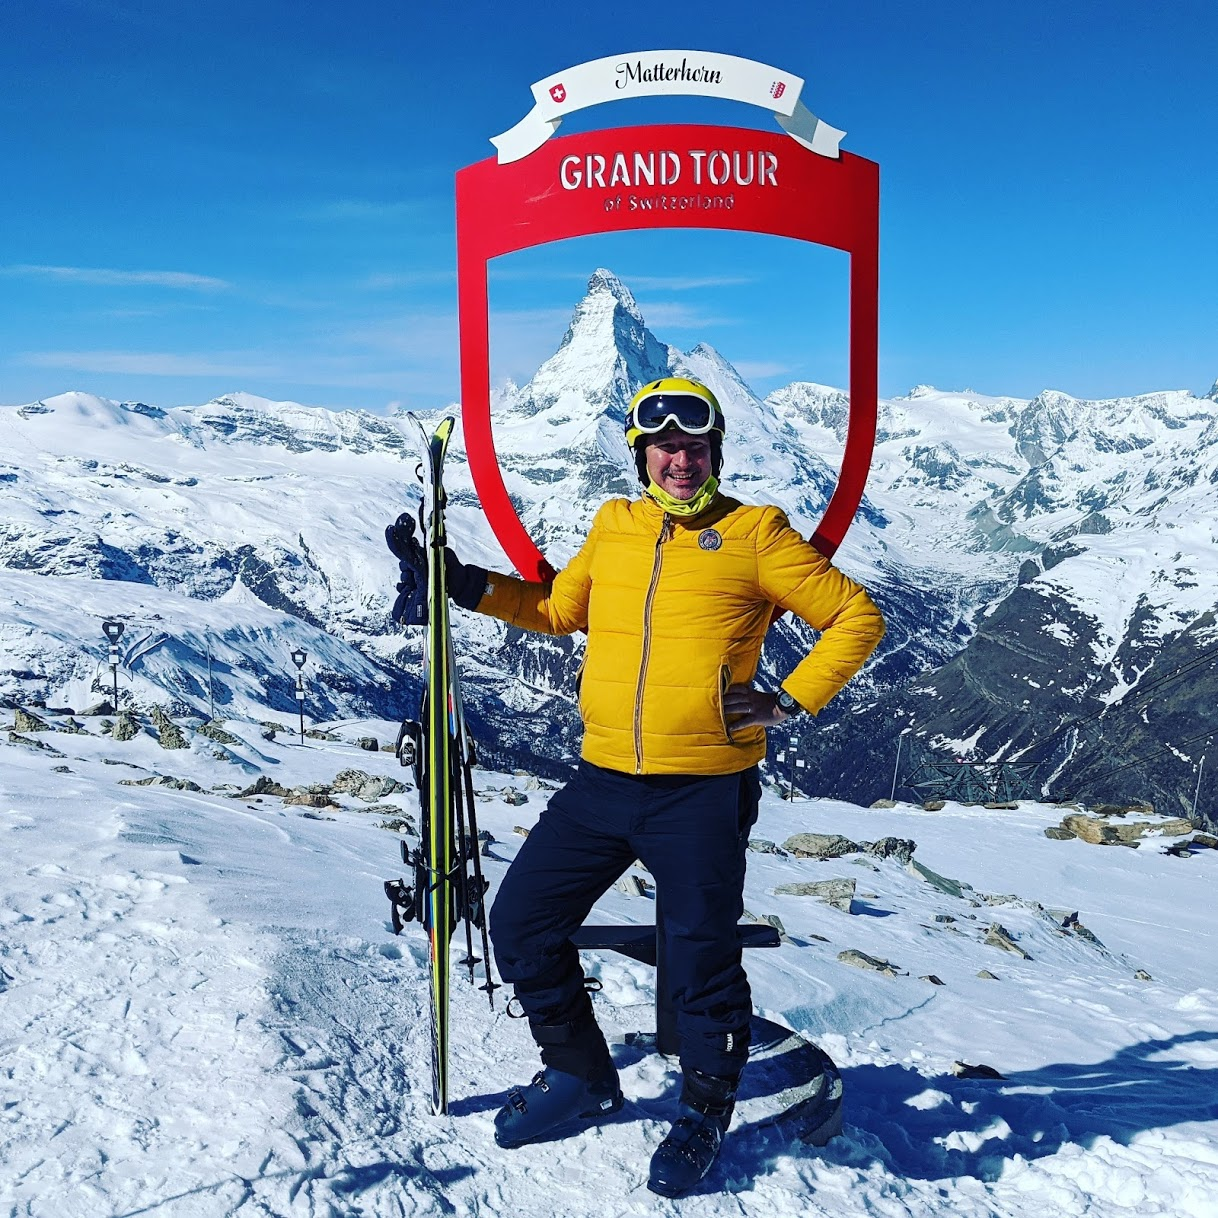
\includegraphics[height = 300pt, width = 300pt]{images/RiccardoMatterhorn.jpeg}

Se vi trovaste su un'isola deserta per qualche anno, una volta messi a posto i bisogni primari, e foste alla ricerca di un hobby, non potreste dedicarvi a ricercare la storia
perche' vi mancherebbero i libri e i dati per studiarla, e correlare eventi; non potreste dedicarvi alla geografia. Potreste probabilmente dedicarvi alla Fisica, ma vi fermereste
abbastanza presto a riscoprire Newton e presumo non potreste andare oltre un certo punto per mancanza di un laboratorio ben equipaggiato; potreste inventare una pila, una doccia,
e sicuramente vi sarebbe utile. Se vi passasse per la mente di studiare la matematica, tutto cio' che vi serve e' un bastoncino e tanta sabbia. L'indomani probabilmente dovreste
riscrivere alcuni passi spazzati via dal vento, ma le conquiste importanti (ad esempio, supponiamo che ieri abbiate riscoperto Pitagora) vi rimarrebbero impresse in mente.
A me personalmente piace giocare con la matematica inventando un problema e cercando di risolverlo con carta e penna, senza altri aiuti - come in un'isola deserta. Ho sviluppato 
per questo motivo un approccio inquisitivo (ma perche' facciamo cosi'? E' davvero l'unico modo di fare cosi' o i Marziani potrebbero farlo diversamente? E se avessi mo 6 dita
invece di 5, quanto varrebbe Pi greco? E il teorema di pitagora varrebbe anche su Marte o su una sfera?).

In questo libro cerco di non dirvi pedissequamente cos'e' un limite o una funzione, ma cerco di spiegare con esempi che - si spera - possano avvicinare persone che fino a ieri 
hanno ODIATO la matematica, magari dissacrando quegli altarini di "aulicita'" che magari ve l'hanno resa antipatica sulla crosta. La matematica per me e' come una noce di cocco: ci 
vuole un cacciavite per aprirla, ed e' difficile la prima volta, ma l'interno e' succoso e pieno di sorprese. Il mio scopo e' fornirvi il cacciavite e mostrarvi quanto succoso sia il contenuto.

\section{Per chi e' questo libro}

Questo libro e' inteso per due categorie di persone: 

1. Persone con la terza media (o piu') che abbiano completato la parte piu' elementare della matematica (somme, sottrazioni, percentuali, qualche funzione a sistema) e siano
curiose di conoscere concetti un po' piu' complessi.

2. Universitari che sono costretti ad affrontare questi concetti complessi.

Cerchero' di insegnare la matematica con toni giocosi, talvolta volgari (e slang bolognese), con l'arrogante ipotesi che questo linguaggio possa essere piu' vicino ai giovani,
e possa insegnare la matematica divertendo. Passero' particolare tempo a spiegare non tanto COSA sia un certo concetto\footnote{Persone piu' brave di me avranno fatto un ottimo
lavoro e saranno disponibili online, se volete definizioni esatte e teoremi ben enunciati.} ma perche' lo studiamo, perche' e' importante, e tutte quelle piccole cose che i
vostri professori hanno probabilmente dato per scontato.

In altre parole cerchero' di fare per la matematica quello che un bravo professore di storia cerca di fare per la Storia: fornirvi il contesto.

E visti gli ultimi tempi con il Covid-19, mi sono accorto di quanto ci sia bisogno di matematica (e statistica) nella vita di tutti per evitare di dire le baggianate che sto ascoltando nei 
social Network. :)

\b{Nota}. Questo "libro" e' stato scritto a internet spenta (probabilmente alla prossima passata mi accertero' di non aver scritto baggianate).

  \label{notazione}
\chapter{Notazione e definizioni}

\citazioneinizioparagrafo{You don't have to be a mathematician to have a feel for numbers	}{John Forbes Nash, Jr.}

In questo capitoletto tratteremo il difficile problema di capirci: non solo quando si parla italiano (il che e' lasciato
alla mia capacita' di scriverlo e a quella delle vostre maestre delle elementarii), ma anche quando si parla matematichese
(con quegli strani simboli come $\forall$, $\nu$, $\doteq$, $|$, \ldots). Questo capitolo vuole in parte spiegare come i
matematici parlano matematichese (80\% circa) e in parte come {\em io} parlo matematichese (il rimanente 20\%).
Tenetelo in considerazione almeno ogni tanto; ora come ora, vi do il permesso di saltarlo, poiche' e' certamente il piu' noioso.

\section{simboli}

\begin{enumerate}
  \item{\b{$\doteq$}} Simbolo di definizione; il $90\%$ delle volte si intende: definisco ci\'o che sta a {\em sinistra} con ci\'o che sta a {\em destra}. Ad esempio: $ x \doteq 2$ vuol dire: definiamo X come il numero 2 (facile),
  mentre con $ f(x) \doteq x$ intendiamo: definiamo come $f$ la funzione che e' uguale a $x$ per ogni $x$, ovvero la funzione identita' (molto piu' coomplesso). Nel primo caso associamo a un acino d'uva il valore 2, nel secondo
  associamo a un grappolo d'uva tanti valori diversi che dipendono da che acino sia. Una nota estetica: non amo questo simbolo perche' non c'e' nulla dentro ad esso che 
  privilegi la sinistra sulla destra, per cui preferico questo simbolo, ad esso equivalente: $:=$
  \item{$\equiv$} Simbolo di equivalenza; $a \equiv b$ vuole dire che $a$ \'e equivalente a $b$ (el $90\%$ delle volte si intende: definisco ci\'o che sta a {\em sinistra}
  con ci\'o che sta a {\em destra}). E' qualcosa di pi\'u forte dell'uguaglianza (so che fa strano, ma pensate a dire $f(x)=g(x)$ e a dire $f(x) \equiv g(x)$: nel primo caso
  cerchiamo di vedere per quali $x$ $f$ e $g$ si ugagliano, nel secondo stiamo dicendo che le due funzioni sono perfettamente identiche). Da notare che il segno di equivalenza 
  tende ad aver senso solo per concetti complessi come funzioni e insiemi che a sinistra e a destra possano avere diversi valori. Per singoli valori come 3 e 4, equivalenza 
  e uguaglianza sono equivalenti (pun intended), quindi e' inutile scomodare l'equivalenza dato che l'uguaglianza ha piu' anzianita'.
  \item{positivo}. Una cosa che spesso confonde e' la definizione di numero positivo: chiameremo un numero positivo un numero come 0,1,2,42. Anche lo 0 e' positivo. Chiameremo 
    un numero \em{strettamente positivo} un numero da 1 in su. Allo stesso modo chiameremo un numero negativo se va da 0 in giu', e strettamente negativo un numero strettamente minore di 0.
    Da notare: 0 e' sia positivo che negativo, ma non e' ne' strettamente positivo ne' strettamente negativo. Il piu' piccolo numero positivo e' 0, ma il piu' piccolo 
    numero strettamente positivo esiste solo per pochi insiemi (come i naturali, che e' 1); buona fortuna a dirmi il piu' piccolo reale maggiore di 0! Se lo 
    trovate, io vi trovo il simbolo, lo chiamero' $0^+$ o $\varepsilon$, ma per favore, ditemi il suo valore esatto ;)
\end{enumerate}

\section{Come leggere una funzione}

% TODO(ricc): forse questo lo puoi spostare al capitolo funzioni.

\subsection{Una funzione facile: una retta}

Cominciamo con un esempio facile. Proviamo adesso a leggere insieme una formula "complessa" e cercare di sfatare i miti.

\begin{equation}
  y = a x + b 
\end{equation}

Oppure (piu esplicita): 

\begin{equation}
  f(x) = a x + b 
\end{equation}

Come leggerla: la funzione $f$ o $y$ e' funzione della variabile X. Quanto vale? Beh, cambiando a casaccio X e assegnadogli valori
come 0, 1, 42, 1000, .. la funzione vi dice che il suo valore sara', rispettivamente: $b$, $a+b$, $42a+b$ e $1000a+b$.

La parte piu' complessa di questa operazione e' capire il ruolo di tutte quelle lettere, per cui faro' uno sforzo a dirlo in modo semplice e chiaro:

* X e' la variabile, e in quanto tale puo' far cio' che vuole. La funzione "itera" 
  (o meglio, si muove) al variare di X e quindi X e' libera di pascolare dove e come meglio crede.
* $a,b$ sono invece dei coefficienti noti. Sono un po' ipocriti, lo ammetto, perche' il matematico sa che i valori sono fissi
  ma invece di dire che valgono, ad esempio, 2 e -3, diciamo semplicamente $a,b$. C'e' un motivo aldila' del sadismo puro:
  in genere se facciamo cosi' e' perche' l'andamento concettuale della funzione non cambia molto al cambiare di a,b. Lo capiremo
  meglio durante lo studio di funzione.

\subsection{Una funzione piu' complessa: un generico polinomio}

Questa e' abbastanza criptica:

\begin{equation}
  f(x)= \sum_{i=0}^n a_ix^i 
\end{equation}

% = a_nx^x+a_{n-1}x^{n-1}+\ldots+a_1x+a_0

Essa va letta come: somma per i (parametro libero di spaziare su N valori) che va da $0$ a $n$ di $a_i$ che moltiplica $x$ alla $i$.

La parte a mio avviso piu' difficile qui e' capire cosa e' un numero e cosa e' una variabile.

Come sempre, siamo in una funzione di $x$ quindi capiamo dal lato a sinistra dell'uguale che la variabile e' la $x$.
E il resto? Cosa sono quei pedici? 
Ebbene, ricordate il caso facile $ a x + b $? Bene, ora iniziamo una discussione virtuale col vostro professore:

- Bene, ora estendila ad una generica equazione di grado due
- Voi: facile, basta aggiungere un X quadro, con un coefficiente a raglio davanti:

\begin{equation}
  f(x)= a x + b + c x^2
\end{equation}

Si pero' e' bruttina (ha i coefficienti a raglio, a,b,c moltiplicano rispettivamente frado 1,0,2, non va bene),
permutiamo i coefficienti e rendiamola piu' leggibile:

\begin{equation}
  f(x)= a x^2 + b x + c
\end{equation}

Molto meglio! Ovvio che in questo caso i coefficienti a,b della retta sono ora b,c, ma poco male.

- Bene, bravo, ora generalizzala ad un'equazione di grado tre:

- Nulla di piu' facile prof, ormai ho capito:

\begin{equation}
  f(x)= a x^3 + b x^2 + cx + d
\end{equation}

- Bene, bravissimo! Ora generalizzala ad un'equazione di grado N:

- Uhm, N? che significa N? Dieci? Di piu'? Beh cosi' a occhio se N fosse anche 100 verrebbe fuori qualcosa tipo:

\begin{equation}
  f(x)= a x^{100} + b x^{99} + ... + v x + z
\end{equation}

Ora ho un problem amolto piccolo, le lettere sono solo 21 (26 se scomodiamo le anglosassoni), ma io ho 101 coefficienti qui,
come faccio? Beh i matematici hanno risolto questo problema con un trucco: invece di scomodare una lettera diversa $a,b,c$ 
usiamo una sola lettera $a$ e la iteriamo da 1 a 100: $ a_1, a_2, a_3, ... a_100 $. Facile no? Possiamo addirittura anche
assegnare $ a_0, a_{-1} $ alla bisogna, purche' siano iterabili (quindi della cardinalita' di $\mathbb{N}$ , non di $\mathbb{R}$). 

Bene, allora un modo piu' elegante di esprimere questa notazione e': 

\begin{equation}
  f(x)= a_{100} x^{100} + a_99 x^99 + ... + a_1 x + a_0
\end{equation}

Ora, se voleessimo fare i pignoli e togliere quei puntini di sospensione che fanno molto "il mio completo elegante e'
in lavatrice quindi sono venuto a fare l'esame in tuta", potremmo scomodare una sommatoria e fare un'ottima impressione: 

\begin{equation}
  f(x)= \sum_{i=0,100}^100 a_i x^i 
\end{equation}

Da notare che qui abbiamo due "variabili": la X che e' la  nostra cara variabile di funzione e la $i$. Si noti che la $i$
serve solo per "sgirellare" la sommatoria, vuol dire: hey tu, si', proprio tu: prendi un generico $i$ che va da 0 a 100 e 
srotolalo al mio segnale. 

* Quando $i$ vale 0, sostituiscila e scrivi quel che vien fuori: $a_0 x^0$ (convenzionalmente $1$), quindi  $a_0$.
  e quindi $a_0$. Wow, questo era strano - vediamo se von gli altri e' piu' facile: 
* Quando $i$ vale 1, $a_1 x^1$ ovvero $a_1 x$. Ok, facile.
* Quando $i$ vale 2, $a_2 x^2$ ovvero $a_2 x^2$. Ok, facile.
* Potrei andare avanti cosi' da 3 a 99 ma non lo faro'.
* Quando $i$ vale 100, $a_100 x^100$ ovvero $a_100 x^100$. Ok, facile. 
* Ora capisco. Mettendo tutti i pezzi insieme vengono: 

\begin{equation}
  f(x)= a_0 + a_1 x + a_2 x^2 + ... + a_100 x^100
\end{equation}

il che e' la versione in tuta del piu' elegante: 

\begin{equation}
  f(x)= \sum_{i=0,100}^100 a_i x^i 
\end{equation}

Ed eccoci da capo.

Come vedete, quando i matematici scrivono queste equazioni criptiche, non lo fanno per sfoggiare (ok, forse un po'..),
lo fanno soprattutto per rendere un concetto complesso con un piccolo numero di caratteri, che definisce \em{precisamente}
quel che vogliono definire. Questa notazione e' fondamentale per esprimere concetti complessi. Voi potreste pensare: ma si'
dai Riccardo, siamo onesti, potevi usare i 3 puntini invece della sommatoria, volevi solo fare lo sborone. In verita' la
risposta corretta e': si', in questo caso particolare i 3 puntini erano sufficienti a far capire questa sommatoria, ma come
avrei potuto spiegare qualcosa di complesso come una sommatoria tripla? Con 3 serie di 3 puntini? E chi itera su chi? Con 
piu' somme, ci saremmo tutti confusi e la versione con $\varSigma$ sarebbe l'unica con spiegazione univoca.

  \label{numeri}
\chapter{Numeri}

\citazioneinizioparagrafo{Per tre punti non allineati passa una ed una sola retta, purche' abbastanza spessa}{Giulio Cesare Barozzi, Lezioni di Analisi III}

\citazioneinizioparagrafo{Perfect numbers like perfect men are very rare}{Rene Descartes}

s%The memoir document class offers "out of the box" commands \chapterprecis, \chapterprecishere, and \chapterprecistoc:
%https://tex.stackexchange.com/questions/53377/inspirational-quote-at-start-of-chapter
%\chapterprecishere{Per tre punti non allineati passa una ed una sola retta, purche' abbastanza spessa\par\raggedleft--- 
%  \textup{Giulio Cesare Barozzi}, Lezioni di Analisi III
%}

In questo capitolo si parler\'a della teoria dei numeri (nella quale son sempre stato poco ferrato): vi dir\'o lo stretto necessario per capire i numeri naturali,
reali, complessi senza la pretesa di dare rigorose specifiche formali degli stessi.

I numeri fondamentali che servono nella matematica sono naturali, interi, razionali, reali e complessi. Cercher\'o di darne una rudimentale definizione,
di fare qualche esempio, e di vederne alcune propriet\'a.

\section{Insiemi notevoli, in breve}

Cominciamo con una carrellata degl'insiemi notevoli (gruppi di numeri con cui ci piace giocare) ed alcune loro proprieta', particolarmente il loro comportamento all'infinito:

* $\mathbb{N}$: Questo e' l'insieme dei \textbf{Naturali}, ovvero {0,1,2,3, .. 42, 100, 1000, 1000000, ... , e tanti altri }. Quelli che in
  italiano chiamiamo numeri interi in matematica si chiamano numeri naturali.

* $\mathbb{Z}$: L'insieme degl'\textbf{Interi} e' simile al precedente ma include anche i numeri negativi. 
 E' grande esattamente il doppio di $\mathbb{N}$, eppure e' grande uguale ad $\mathbb{N}$ \footnote{Eh gia', strana cosa gli infiniti. Si puo' dimostrare che la cardinalita' di N e Z sono uguali, e le sorprese non sono finite.. }.
 I numeri che contiene sono $0,1,-1,42,-42,1000,-1000$, e cosi' via.

* $\mathbb{Q}$: Questo e' l'insieme dei \textbf{Razionali}, ovvero l'insieme dei numeri frazionari espriminbili come $\frac{p}{q}$.
Alcuni esempi sono: $1,2/5,3/4,-42$ . Da notare che i razionali contengono gli interi ma contengono moltissimi piu' numeri.
E' un insieme molto denso nel senso
che tra i suoi 2 valori $1/10$ e $2/10$ ci sono infiniti valori. La cosa forse piu' incredibile e' che (Peano lo dimostro' per primo)
la cardinalita' di $\mathbb{Q}$ e la stessa di $\mathbb{N}$. Lo so, assurdo. Eppur vero. L'infinita' di questi interi e infiniti ad essa
isomorfi e' di difficile comprensione, ve lo concedo.

* $\mathbb{R}$: insieme dei \textbf{reali}. Chiameremo $\mathbb{R}+$ l'insieme dei reali >= 0 e con $\mathbb{R}-$ i reali con x<=0, e con $\mathbb{R}*$ l'insieme dei reali $senza lo \{0\}$.

* $C$: insieme dei \textbf{complessi}. I complessi meritano un capitolo a parte. L'insieme \egrave isomorfo a $R^2$ (ovveri tutti i punti in un piano).

* $\mathbb{R}^3$: insieme di terne di reali. In matematica non esiste ma in fisica si usa un casino per definire la posizione di un punto nello spazio
e ci tenevo a contestualizzarlo qui.

* $\mathbb{Z}_p$: insieme di di interi modulo $p$. Questo insieme si dice anello, e gode di interessantissime proprieta' ma e' difficile parlarne se non decidiamo $p$. 
  Se $p$ e' un numero primo, gode di ulteriori proprieta' ad esempio la possibilita' di inversione per la moltiplicazione. Esempio: $\mathbb{Z}_5 := {1,2,3,4,5}$ o ancora
  meglio $\mathbb{Z}_5 := {0, 1,2,3,4}$. Si', la cosa incredibible di questo insieme e' che 0 e 5 sono la stessa cosa, quindi intercambiabili. Un professore bastardo
  potrebbe addirittura dirvi che $\mathbb{Z}_5 := {420, -4, 427, -42, 420004}$. Se dividete un numero per 5 e guardate al resto, 1 e 6 e 66 sono la stessa cosa, no? 
  Per maggiori informazioni: \href{https://it.wikipedia.org/wiki/Aritmetica_modulare}{Aritmetica modulare su Wikipedia}.

\section{I numeri naturali}

Tutto nasce dai naturali. Schiere di filosofi e matematici hanno provato a darne una definizione. Peano e Russell (se ben ricordo) ne hanno dato una definizione operativa che vi propongo.

- Esiste un numero iniziale che chiameremo $zero$ ($0$).

- Per ogni numero naturale $N$ esiste un successore, che chiameremo $s(N)$ (\'e una funzione, se ci si pensa).\footnote{Quindi $1=s(0),2=s(s(0))$, e cos\'i via. 
No, non vi invito a scrivere 1000 in questa notazione.}.

- Mi pare vi siano altre propriet\'a, ma non mi vengono in mente.

Ora, si pu\'o tranquillamente fare matematica in queso modo, per esempio il famoso $2+2=4$ diventa $s(s(0))+s(s(0))=s(s(s(s(0))))$. Capite pero' che per scrivere $12*12=144$ servirebbero tante righe e per $1'000*1'000=1'000'000$ 
servirebbero intere pagine. Ecco perch\'e la notazione 'posizionale' che tutti conosciamo (10=dieci, 100=cento, 110=centodieci) torna utile per risparmiare inchiostro. Quando capirete che la matematica sfrutta ogni possibile strada
per risparmiare inchiostro, comincerete a pensare come dei veri matematici...

Una interessante propriet\'a dei naturali \'e che non hanno un limite destro, per cui si dice che vanno all'infinito. Vi sono anche studi su $quanti$ siano i naturali.
L'infinit\'a dei naturali viene detta $\aleph_0$, ed \'e la pi\'u piccola infinit\'a conosciuta. Ebbene s\'i, ci sono tanti infiniti, alcuni pi\'u grandi, alcuni pi\'u piccoli.

Denoteremo con $\insieme{N}$ l'insieme dei naturali: $\insieme{N}\cdot\{0,1,2,3,4\ldots\}$


\section{I numeri interi}

Tutti pensano che gl'interi siano i naturali. In matematica, invece, i naturali sono i numeri interi "positivi", men tre si chiamano $interi$ i numeri interi positivi o negativi.
Credo che la definizione sia:

- Esiste lo zero ($0$).

- Per ogni $z$ esiste un successore $s(z)$.

- Per ogni numero $z$ esiste l'opposto $-z$.

L'insieme che viene fuori \'e: $\insieme{Z} \cdot \{0,1,-1,2,-2,3,-3,\ldots\}$. Attenti, potevo anche dire che l'insieme \'e: $\{\ldots,-3,-2,-1,0,1,2,3,\ldots\}$.


\section{I numeri reali}

I numeri reali sono espressi come numeri che possono essere definiti come limite di una successione di razionali. E' davvero buffo pensare che sommando ingredienti tutti razionali dal primo all'ultimo (e potrete immaginare che la somma di due razionali sia sempre razionale!) possa dare come risultato qualcosa che \em{ non} sia razionale.


\section{I numeri complessi}

\b{Introduzione}.
I numeri complessi sono numeri molto interessanti perch\'e ci si \'e arrivati ben dopo agli altri numeri e ci si \'e accorti della loro esistenza a causa di "buchi" nella matematica comune 
che non potevano essere spiegati in altro modo. La genesi di questi numeri, a quanto ne so, nasce dalla necessita' di trovare soluzioni a equazioni polinomiali di grado $N$. ci si \'e infatti
accorti che la soluzione di un'equazione polinomiale di grado 3 (ad esempio) e' spesso data da 3 numeri, ma talvolta da uno solo. E le soluzioni di un'equazione di grado 7 possono essere 7,5,3 oppure 1.
Se ci inventiamo questo mondo "fittizio" dove facciamo finta che la radice quadrata di $-9$ abbia un senso, ecco che quasi per magia si scopre che in questo mondo favoloso le soluzioni di un'equazione
di grado N sono sempre N! Quindi restate con me se la cosa vi incuriosisce, come incuriosisce me.
 


  \label{funzioni}
\chapter{Funzioni}

In questo capitolo si parler\'a di funzioni. Nella prima parte ne verranno dati definizioni ed esempi, 
nella seconda si parler\'a dello 'studio di funzione', e nella terza si affronteranno tanti piccoli temi
collaterali. Ho speso molte parole per spiegarne il concetto poich\'e \'e a mio parere uno dei pi\'u 
affascinanti e complessi della matematica: l'uomo riesce con facilit\'a a ragionare su numeri, ma su qualcosa
che associa infiniti numeri a infiniti numeri tende ad avere sempre delle perplessit\'a. Molto spazio verr\'a
dato alle funzioni notevoli, poich\'e \'e a partire da questi mattoncini che si costruiscono quei maestosi
castelli che i professori mettono nei vostri compiti...

%\prerequisito{Dovete guardare prima i grafici.}

\section{Cos'è una funzione}

Cosa è una {\em funzione}? Essa \'e una applicazione che associa tutti 
i valori di un dominio (ovvero un insieme $\mathbf{X}$) a certi valori su un 
codominio $\mathbf{Y}$ (un altro insieme).
\begin{equation}
f: x \in \mathcal{X} \mapsto \mathcal{Y}
\end{equation}

Detto in parole pi\'u povere, {\em \'e un oggetto 
che mangia numeri e sputa fuori numeri in maniera prevedibile}. Se gli date da 
mangiare una stessa cosa (per esempio $x_0:=46,2$) e lui 'gradisce' questa 
cosa (ovvero $x_0$ è contenuta nel dominio $\mathcal{X}$), la funzione 
sparer\'a sempre fuori uno stesso numero. Esso \'e detto $f(x_0)$. Il concetto di funzione
è molto importante poichè è quanto di pi\'u generale ci sia: una funzione pu\'o 
mangiare qualunque cosa e 'spararla' in quasi qualunque altra cosa. Ci\'o che \'e pi\'u
difficile da capire \'e che il nome della funzione \'e indipendente da quello che le 
si d\'a in 'ingresso'.

Vediamo di inventarci qualche funzione per fissare il concetto.

\begin{equation}
% f(x) \doteq x+3; 
%\end{equation}
%\begin{equation}
 f(0) \doteq 3; \\
 f(1):=4; \\ 
 f(2):=5; \\ 
 f(-5):=-2; \\ 
  \ldots
\end{equation}

La funzione che ho scritto potrebbe essere qualunque cosa; probabilmente la pi\'u
semplice funzione che si comporti come lei \'e: $f_1(x)=x+3$\footnote{Ma attenti,
esistono un bel po' di funzioni che rispettano questi vincoli. E' un po' come cercare
moglie secondi i vincoli: '2 occhi', '2 seni', 'che respiri'. Un altro esempio, solo per persuadere
i pi\'u scettici, \'e $f(x)=4+sen(\frac{\pi}{2}(x-1))$}. Non bisogna sottovalutare 
la \emph{potenza} di questa notazione, per cui prendiamoci un po' di tempo per 
capirla. Quando scrivo $f(x \in \mathbf{R})=x+3$ intendo un oggetto che, dato un numero, 
vi risponde con un altro numero. In ingressso dovete dargli un numero reale e in uscita 
vi restituir\'a un altro numero reale. Per capirci meglio, daremo d'ora in poi a $f$ il 
simpatico nome di '{\bf sommatre}'

Mi piacerebbe spiegarvi le funzioni in un modo alternativo, come me lo spieg\'o il mio prof
di Geometria, Massimo Ferri nel 1995. Pensate di avere un asse orizzontale in cui \'e libero di muoversi un cannone;
esso pu\'o sparare solo in verticale, su o gi\'u, ma sempre in verticale rispetto a dov'\'e. Ora
immaginate che il cannone sia programmato per sparare sempre in un medesimo punto (esempio in $3$)
se si trova in una certa posizione (ad esempio $0$). Se il cannone si trova nel punto $-5$ (che sta
ad ovest, per intenderci), sparer\'a sempre in basso all'altezza di $-2$. Infine, quando si trova
in $-3$, si spara addosso, ma questo non \'e un problema che ci tocchi. Se dopo aver istruito il
cannone su come sparare, lo fate andare all'infinito a destra e a sinistra, potrete osservare la scia
che lascia su un ipotetico foglio di carta; questa \'e il {\em grafico} della funzione. Cos'\'e la 
funzione? L'equazione? Il grafico? Il carroarmato? No! Essa \'e l'insieme di istruzioni che avete dato al carroarmato.
Ci\'o che pi\'u si avvicina alla sua definizione senza perdere infiniti fogli a scrivere $f(0,1,2,3,\ldots)$ \'e
la parola 'sommatre'; ma attenti: se la funzione si complica non sempre avrete la fortuna di poterle dare un nome semplice
quindi dovrete adeguarvi alla notazione usata in quei noiosissimi libri di matematica. Ma prima di arrivare a quella notazione,
cerchiamo di capire il senso dietro ad essa.

E' importante capire che la funzione {\bf sommatre} \'e qualcosa che somma tre al numero 
che le date in pasto. Alcune domande {\em ben poste} potrebbero essere: quanto vale $f(0)$? Per quale
 $x$, $f((x)$ vale 15? Quando \'e massima $f$? Quand'\'e che $f$ incontra gli assi cartesiani? 
 Per quali valori del dominio $\mathcal{X}$  $f$ \'e definita? 
 \footnote{Alcune domande mal poste potrebbero essere: 's\'i ok $f(x)$, ma questa benedetta $x$ quanto cacchio vale?!?'}.
 
Tutte queste sono domande che vi potrebbero essere fatte quando vi si chiede di fare lo \em{studio di funzione} di $f$. 

Mi ritengo soddisfatto se sapete rispondere (per iscritto) a queste domande a trabocchetto: {\bf Che cos'\'e $f(x)$? Che cos'\'e $f(t)$? Che cos'\'e $f(0)$?}  

Una risposta pu\'o essere: le prime due sono \em{funzioni} (per la precisione sono sempre la nostra amica 'sommatre'), la terza \'e un \em{numero} (ed \'e il numero $3$, poich\'e $0+3=3$:
provatelo con le vostre calcolatrici tascabili). Ma allora che cos'\'e $x$? E che differenza c'\'e tra $x$ e $t$? Questa credo sia la domanda pi\'u difficile che ci si possa fare sulle
funzioni. Una buona risposta \'e che la $t$ \'e la $20^{ma}$ lettera dell'alfabeto anglosassone mentre la $x$ \'e la $24^{ma}$.. a parte la battuta il fatto \'e che non c'\'e alcuna differenza
tra $f(x)$ e $f(t)$, se non il fatto che nel primo caso $f$ dipende da $x$ e nel secondo da $t$: la variabile \'e muta di per se stessa,
e ha senso \b{solo} nella definizione stessa della funzione\footnote{La cosa diventerebbe rilevante in qualcosa
come: $f(x)=3tx$, in tal caso $x$ \'e la variabile e $t$ sar\'a probabilmente un parametro.}; ma la funzione sar\'a
sempre lei, nel nostro caso sar\'a sempre 'sommatre', ovvero qualcosa che mangia un numero, gli somma 3 e sputa fuori
il risultato. Un altro modo per capirlo, \'e inventarsi un mondo senza $x$; proviamoci per un attimo. Prendiamo la nota
funzione $f(x)=x^2+2x+1$; prima dell'ottocento, i matematici la leggevano come 'prendi un numero, elevalo al quadrato,
poi aggiungi il doppio del numero e infine aggiungi uno'. Capirete che se un prof vi chiede se questa sia una parabola
o un'iperbole farete abbastanza fatica a rispondergli, no? Allora diremo: $f(numero)=numero^2+2 \cdot numero+1$.
Ancora troppo lungo. Proviamo con la $x$: $f(x)=x^2+2x+1$. Oh! Ora va meglio.

Scusate la lunghezza della digressione, ma dopo anni e anni di matematica, vedo persone ancora perplesse sul vero
significato della fatidica \em{variabile indipendente}. Potete pensare che $x$ sia una variabile \em{muta},
assolutamente inutile, e quindi il vero modo per chiamare la nostra amica 'sommatre' in modo matematico non sia $f(x)$,
bens\'i $f(\dot)$\footnote{credo che l'unico modo di apprezzare una funzione per ci\'o che \'e sia proprio quella di
usare un puntino, del tipo $f(\cdot)=\frac{\cdot+1}{1+\cdot^2}$; ovvio che se usate una $x$ al posto di $\cdot$ si legge
meglio, no?}. Ricordate: se scrivo $f(x)=x+3$ e $g(y)=y+3$, definisco la stessa funzione: $f$ e $g$
sono {\em perfettamente identiche}!!! O se preferite $f(Franca)=Franca+3$ e $g(Iolanda)=Iolanda+3$.
D'ora in poi, per\'o, preferiremo chiamare $x$ ci\'o che la $f()$ mangia e $y$ ci\'o che la $f$ sputa,
e al posto della $x$ useremo $t$ se penseremo a tempi o $\theta$ se pensiamo ad angoli: i matematici ci
tengono molto a dare significati diversi alle diverse lettere, e ne hanno cos\'i tanti che le 26 dell'alfabeto
anglosassone non bastan loro, e devon tirarne fuori anche da quello greco ed ebraico...

Vi faccio un esempio stupido: quando davanti a una birra un amico/a mi dice "Sai Riccardo, mi e' capitato X volte ...." il mio
volto si scurisce perch\'e ho la certezza che la persona davanti a me non abbia studiato o apprezzato la matematica
quanto me. Cos\'i come abbiamo l'archetipo delle Susan e dei Dick in inglese, cos\'i abbiamo l'archetipo delle lettere:

* a,b,c sono parametri/coefficienti
* x,y,z sono variabili reali
* i,j,k,l,m,n sono variabili intere 
* $\alpha , \beta , \gamma$ sono coefficienti pi\'u eleganti di a,b,c. Talvolta usati in congiunzione/parallelo (a vs alpha, ..)
* $\theta, \vartheta, \phi$ sono angoli 

Come avrete capito, l'amico avrebbe dovuto usare N e non X per avere la mia stima :) E s\'i, ovviamente la persona bacata nel cervello sono io, non l'amico. 

\section{Funzioni notevoli}
In questa sezione cercher\'o di analizzare le funzioni pi\'u famose. La maggior parte delle funzioni che vi cappiter\'a di studiare
saranno 'case' costruite con questi mattoncini... Per ciascuna funzione cercher\'o di evidenziare le caratteristiche pi\'u
interessanti di ciascuna, tra cui il grafico (un giorno), derivate, primitive, estremanti, poli, ..

\subsection{Polinomi}

Un polinomio \'e una equazione nella forma:

\begin{equation}
f(x)= \sum_{i=0}^n a_ix^i = a_nx^x+a_{n-1}x^{n-1}+\ldots+a_1x+a_0
\end{equation}

Alcuni esempi di funzione sono: $x^42+37x+41$,$3x^2+6x+3$, $x^2+1$, ma non $\frac{1}{x^2+1}$. Attenzione, anche $3-x$ e $5$
(una delle mie funzioni preferite, l'avrete notato) sono polinomi, e questo la gente tende a dimenticarlo spesso...

Attenzione, come sempre le $x^n$ sono potenze della nostra amica variabile indipendente, mentre le varie $a_0,a_1,\ldots$
sono il DNA del polinomio stesso (non mi credete? Andate a leggervi il capitolo su Taylor, \refpagref{taylor}). Capiamolo con un esempio
stupido: in $x^2+3x+41$ $a_0=41;a_1=3;a_2=1;a_3=0;a_4=0;a_5=0;a_6=0;\ldots$. Se non vi offendete mi fermo qua,
dicendovi che da $a_3$ in poi tutti i coefficienti son nulli. Si dice allora che il polinomio \'e di grado $2$
poich\'e \'e alla posizione $2$\footnote{che \'e al terzo posto, ma ai matematici piace complicarsi la vita,
e spoiler alert! Quasi sempre hanno ragione loro...} che c'\'e l'{\em ultimo} valore non nullo. \footnote{Un modo
molto elegante per definire il polinomio \'e di identificarlo la lista ordinata $(41,3,1)$. Ancora una volta, 
\'e scomparsa la $x$, che guarda caso \'e l'unica cosa non importante per il polinomio!}

\begin{description}
	\item{Dominio} I polinomi non han problemi di dominio: tutto $\insieme{R}$ va bene.
	\item{Codominio} Bazza: se ponete $x=0$ si annulla tutto meno il termine noto, quindi $f(0)=a_0$.
	\item{Zeri} Tanti. In realt\'a ce ne possono essere tanti quanti il grado del polinomio, ma se non avete
	gli 'occhiali' complessi ci possono essere coppie di soluzioni (complesse coniugate) che non potete vedere.
	Esempio: un polinomio di terzo grado ha o $3$ o $1$ soluzioni. Esiste bun trucco per calcolare le soluzioni
	di un polinomio di secondo grado \footnote{Il famoso $x=\frac{-b \pm \sqrt{b^2-4ac}}{2a}$}, un altro per le
	equazioni di terzo e quarto grado, e - se non sbaglio - \'e stato dimostrato che non possono esistere trucchi
	per i polinomi di grado oltre al quarto. {\em Attenti alle molteplicit\'a: $f=x^4+x$ ha 4 zeri: $(0,0,0,-1)$;
	$-1$ \'e uno zero normalissimo, mentre $0$ (che solo per caso si pronuncia allo stesso modo) \'e uno zero di
	molteplicit\'a tripla. Questo \'e molto importante: quando ad esempio una funzione ha uno zero doppio tende
	non solo a passare per il punto ma a esservi tangente (ovvero arrivarci da sotto, toccarlo, e tornar gi\'a
	proprio in quel punto - o viceversa). In generale, non trascurate la molteplicit\'a nei vostri scritti: certe
	persone ci tengono molto ;).}
	\item{Poli} Nessuno.
	\item{Derivata, massimi e minimi} E' molto facile e divertente derivare polinomi. Per la propriet\'a di linearit\'a,
		possiamo derivarla a pezzi, ovvero vale la comodissima propriet\'a che la derivata della somma \'e uguale alla somma
		delle derivate. Se sapete derivare un generico pezzettone $x^n$ (che fa $nx^{n-1}$), sapete derivare tutto. Vien
		fuori: $f'(x)=\sum_{i=1}^n i \cdot a_ix^{i-1} = na_nx^{n-1}+(n-1)a_{n-1}x^{n-2}+\ldots+2a_2x+a_1$. Fate attenzione
		che \'e scomparso il termine noto $a_0$. Il nuovo polinomio ha un grado in meno dell'originale, a meno che non
		avesse grado zero (nel qual caso rimane zero). I massimi/minimi saranno tanti, fino a $n-1$. Calcolate la derivata,
		e di essa calcolate gli zeri. (Io dico sempre: lo studio di funzione di un polinomio \'e per il $60\%$ studio degli
		zeri di $f$, per il $40\%$ studio degli zeri di $f'$: rimane ben poco ancora di interessante).
	\item{Primitiva} Anche qui \'e molto facile, se sapete qual \'e una primitiva dei mattoncini $x^i$ (che \'e $\frac{x^{n+1}}{n+1}$).
		Viene fuori: $F(x)=\sum_{i=0}^n \frac{a_i}{i+1}x^{i+1}+37 = \frac{a_n}{n+1}x^{n+1}+\frac{a_{n-1}}{n}x^{n}+\ldots+\frac{a_1}{2}x^2+a_0x+37$.
		Il $37$ l'ho aggiunto io per ricordarvi che le primitive son tante, e nessuna ha una dignit\'a maggiore delle altre. Se volete usare
		quella col $+0$ anzich\'e quella col $+37$, avete il mio permesso: io farei lo stesso.
\end{description}


\subsection{$\sin(x)$}

La funzione seno (una delle mie preferite) \'e una funzione trigonometrica. Essa \'e periodica, di periodo $2\pi$. Ci\'o
vuol dire che potete disegnarla e studiarla da $0$ a $2\pi$ (ma anche da $7\pi$ a $9\pi$!) perch\'e si ripeter\'a all'infinito con lo stesso
andamento. Ci limiteremo a studiarla su $[0,2\pi]$. Per una definizione pratica di seni e coseni rimando al capitolo su di essi
(\refpagref{trigonometria}). Capirete che una funzione come questa se ha uno zero ne ha infiniti, se ha un polo ne ha infiniti e cos\'i
via... Mi limiter\'o al solo intervallo $[0,2\pi[$. Spesso potrebbe capitarvi di studiiare invece $]-\pi;\pi]$

\begin{schedaf}
	\rigaf{Dominio}{Tutto $\insieme{R}$.}
	\rigaf{Codominio}{E' piccolissimo: $[-1;1]$}
	\rigaf{Zeri}{$0,\pi$}
	\rigaf{Poli}{Nessuno.}
	\rigaf{Derivate}{$D\sin(x)=\cos(x)$. Massimo: $\frac{\pi}{2}$. Minimo: $-\frac{\pi}{2}$}
	\rigaf{Integrali}{$\int\sin(t)dt=k-\cos(x)$. Aree: $A_S[0;\pi]=2$ \footnote{L'area del periodo \'e 4, ma l'integrale \'e nullo: vedi studi di funzione sugli integrali}.}
	\rigaf{Altro}{La funzione e' periodica di periodo $2\pi$.}
	\rigaf{Punti notevoli}{$f(0)=0;f(\pi/2)=1;f(\pi)=0;f(3\pi/2)=-1$.\footnote{Ce n'\'e altri, ma per essi rimando il capitolo ad essi dedicato.}}
\end{schedaf}

\subsection{$\cos(x)$}
Come il seno \'e periodica di periodo $2\pi$: useremo, tanto per allenarci, l'intervallo $]-\pi;\pi]$.
\begin{schedaf}
	\rigaf{Dominio}{Tutto $\insieme{R}$.}
	\rigaf{Codominio}{$[-1;1]$}
	\rigaf{Zeri}{$-\pi/2,\pi/2$}
	\rigaf{Poli}{Nessuno.}
	\rigaf{Derivate}{$D\cos(x)=-\sin(x)$. Massimo: $0$. Minimo: $\pi$.}
	\rigaf{Integrali}{$\int\cos(t)dt=k+\sin(x)$}
	\rigaf{Altro}{La funzione e' periodica di periodo $2\pi$.}
	\rigaf{Punti notevoli}{$f(0)=1;f(\pi/2)=0;f(\pi)=-1;f(-\pi/2)=-0$.}
\end{schedaf}

\subsection{$\tan(x)$}
La tangente altri non \'e che $\frac{\sin(x)}{\cos(x)}$, e ne eredita la periodicit\'a. Anzi, \'e addirittura periodica di periodo $\pi$ (il che non inficia la frase prededente, rifletteteci). La studieremo su $]-\novanta;\novanta]$.
\begin{schedaf}
	\rigaf{Dominio}{$]\-novanta;\novanta[$; \footnote{C'\'e un unico buco in $\novanta$ che significa infiniti buchi a distanza $\pi$!!!}}
	\rigaf{Codominio}{Tutto $\insieme{R}$.}
	\rigaf{Zeri}{$0$}
	\rigaf{Poli}{$\novanta$}
	\rigaf{Derivate}{$D\tan(x)=\frac{1}{\cos^2(x)}=1+\tan^2(x)$ (come preferite). Massimi/minimi: nessuno.}
	\rigaf{Integrali}{$\int\tan(t)dt=k-\log|cos(x)|$}
	\rigaf{Altro}{La funzione e' periodica di periodo $\pi$.}
	\rigaf{Punti notevoli}{$f(0)=0;f(\pi/4)=1;f(\pi/2^-)=+\infty;f(-\pi/2^+)=-\infty$.}
\end{schedaf}


\subsection{Funzioni iperboliche ($\sinh(x)$, $\cosh(x), ..)$}

Le funzioni iperboliche sono fondamentalmente degli esponenziali che puzzano dannatamente di funzioni trigonometriche.
Se li disegnate, o li derivate, sono proprio degli esponenziali. Se li guardate al microscopio (con le serie di Taylor (\refpagref{taylor})),
troverete delle inquietanti somiglianze con i 'cugini' trigonometrici (seno con seno iperboolico, coseno con coseno iperbolico,
e soprattutto tangente e tangente iperbolica). La cosa pi\'u buffa \'e che le funzioni sono completamente diverse (ad esempio,
le iperboliche vanno spesso all'infinito e sono aperiodiche mentre le trigonometriche sono spesso limitate tra $-1$ e $1$ e
sono periodiche). Vediamone la definizione.

\begin{eqnarray}
 \sinh(x) := \frac{e^x-e^{-x}}{2}
 \cosh(x) := \frac{e^x+e^{-x}}{2}
 \tanh(x) := \frac{sinh(x)}{cosh(x)} \bigg( = \frac{e^x-e^{-x}}{e^x+e^{-x}}\bigg)
\end{eqnarray}

Le funzioni inverse di queste tre funzioni iperboliche sono facilmente esprimibili con logaritmi. Riuscite a trovarle?

\begin{esercizio}
 Ricavate la funzione $arcsinh(x)$ e le sue sorelle. {\em Hint: $y=arcsinh(x) \Rightarrow x=\frac{e^y-e^{-y}}{2}, ponete \theta=e^y, \cdots$. Dovrebbe venir fuori qualcosa con logaritmi e radici quadrate mi pare.}
\end{esercizio}

Provate un po' a derivarli: cosa notate di strano? 

\subsection{$e^x$}

Che cos'\'e l'esponenziale ($e^x$)? E' una particolare funzione che viene usata tantissimo in tutti i campi dell'analisi, dell'ingegneria, della fisica; perch\'e?
Credo la sua importanza sia dovuta al fatto che sbuca fuori magicamente dalla Equazioni Differenziali. Prima di andare avanti, vi consiglio di guardare la sezione
sugli esponenti (\sezpagsez{fattoriali}).

Come si calcola un esponenziale? Se l'argomento \'e intero, lo pu\'o fare chiunque sia dotato di addizione e moltiplicazione. Negli altri casi, la faccenda si
complica e richiede anche le radici (quadrate, subiche, ...). Vediamo una defizizione ridondante sufficiente a definire gli esponenziali 'di esponente intero' (poniamo $a \ne 0$):
\begin{eqnarray}
a^0 \doteq 1\\
a^{n+1} \doteq a \cdot a^n\\
a^{-n} \doteq \frac{1}{a^n}
\end{eqnarray}
 
 Da questa definizione, segue che $10^0=1, 10^1=10, 10^2=100, 10^3=1000, \cdots, 10^{-1}=\frac{1}{10},10^{-2}=\frac{1}{100}, \cdots, \ldots$. Come vedete questa funzione cresce in fretta: $f(9)$ vale un miliardo, $f(18)$ vale un miliardo di miliardi e $f(-27)$ vale un miliardesimo di miliardesimo di miliardesimo\footnote{Come si pronuncia $f(-16)$?}. 
 Questa funzione \'e sicuramente la pi\'u veloce di tutte le colleghe (potete immaginare quindi il comportamento della sua funzione inversa, il logaritmo...). Ora vediamo di capire la parte in mezzo
 
Per capire $e^x$ credo dovremo cominciare da qualcosa cui siete pi\'u familiari, tipo la funzione (molto simile) $10^x$ (che si legge $10 alla x$). 

\subsection{$\log(x)$}

TBDs 

Notiamo anzitutto che la derivata di $\ln(x)$ coincide con quella di $\ln|x|$. Se guardate i grafici,
vi accorgete che a destra vale $ln(x)$ e a sx dell'asse y $-\ln(x)$. Qui il valore assoluto pu\'o essere visto come un 'completamento naturale di dominio'.

%\subsection{Funzioni iperboliche?!?}
% skippo va
%tbds

\section{Studi di funzione}

Cosa vuol dire \em{studiare} una funzione? Vuol dire semplicemente dire tante cose interessanti di una funzione.
Supponiamo che il vostro prof di matematica vi porti in centro citt\'a il sabato pomeriggio e vi proponga qualcosa
di simile: lo {\em studio di persona}. Vi addita un passante e vi dice: cosa puoi dirmi di lui? Voi direte:
\'e alto $1,70$ circa, pesa sui $70 kg$, ha una corporatura media, i capelli mori ricci e porta gli occhiali;
ha un neo vicino alle labbra e ha dei seni particolarmente grossi. C'\'e qualcosa di non banale in ci\'o che
avete detto: l'altezza, il peso, il colore dei capelli, degli occhi eccetera sono caratteristiche di \em{qualsiasi}
persona. Gli occhiali, i nei, lentiggini, eccetera sono invece caratteristiche di \em{alcuni} individui, eccezioni
della cui presenza ci si accorge ma la cui assenza passa inosservata. Difficilmente direte: "senza occhiali",
"senza barba", "senza n\'ei visibili", o sbaglio? (Ovvio che alla polizia direte anche queste cose se si tratta di un ricercato!)

Lo studio di funzione \'e qualcosa di molto simile: si tratta di delineare una funzione (come la nostra amica 'sommatre')
secondo alcune caratteristiche comuni a {\em tutte} le funzioni, e di trovare quei tratti della funzione che sono interessanti.

\subsection{Dominio e codominio}

La prima cosa da studiare in una funzione \'e sicuramente il dominio di definizione della funzione stessa, ovvero l'insieme
di valori (le $x$, per intenderci) su cui la funzione \'e definita. Alcuni esempi:

\begin{equazione}
 f_1(x)=3x^4-2x^3+87x-57\pi \\
 f_2(x)=\sin(x) \\
 f_3(x)=\log(x) \\
 f_4(x)=\sqrt(x+1) \\
 f_5(x)=\frac{(x-29)(x+3)}{(x-29)(x-12)(x-1976)} 
\end{equazione}

I casi pi\'u complicati sono certamente i primi due: teniamoli dunque per ultimi. Se conoscete la funzione logaritmo, sapete che essa \'e
definita solo per $x>0$, quindi il $\mathcal{D}_{f_3}=\{\mathbf{R} \senza \mathbf{R}^-\}$. Attenti alla pignoleria: $\mathbf{R}^+$ comprende
lo zero, quindi un modo carino \'e prendere tutto $\mathbf{R}$ e togliergli $\mathbf{R}^-$, liberandomi in un sol colpo dei numeri negativi e dello zero.
Il caso $f_4$ \'e molto simile: la radice quadrata esige un argomento non negativo (ovvero i numeri minori di zero le sono indigesti). Attenti per\'o
all'argomento: non c'\'e $x$ questa volta, ma una funzione {\em molto} pi\'u complicata: $x+1$. Abituatevi a ci\'o: per calcolare il dominio della
funzione dovete imporre che l'argomento sia non negativo, il che produce la seguente equazione: $x+1 \ge 0$. Dunque $\mathcal{D}_{f_4}=\{x|x \ge -1\}$.

Il caso $f_5$ vi capiter\'a spesso. Come sapete dalle elementari, la funzione {\em divisione} non accetta un divisore (che
\'e la parte che sta dopo il diviso) uguale a zero, quindi se avete che la vostra funzione \'e uguale a
$f(x)=\frac{qualcosa}{Pippo \cdot Bluto}$ dovrete imporre che {\em sia} Pippo {\em sia} Bluto siano diversi da zero.
Ci\'o significa, nel nostro caso particolare, imporre $x$ diverso da quei tre numerini presi {\em assolutamente} a caso:
$\mathcal{D}_{f_5} = \mathcal{R} \senza \{12;29;1976\}$. Un appunto: quei tre numeri hanno assolutamente la stessa dignit\'a,
e non ne viene uno prima dell'altro (lo dico perch\'e molta gente pensa il contrario).

Veniamo ora ai primi due: vedete qualche pezzettone di funzione che vi faccia scattare un qualche allarme? Vedete poli, radici,
logaritmi, o cose del genere? No, dunque il dominio delle prime funzioni \'e proprio $\insieme{R}$.

In generale, studiare il dominio di una funzione vuol dire partire da $\insieme{R}$, e poi cominciare a stringerlo per ogni
funzione strana che c'\'e l\'a dentro, introducendo le limitazioni della funzione (logaritmi, equazioni fratte, radici, etc).

Parliamo ora di {\bf codominio}. Il codominio \'e l'insieme di valori che la funzione produce.

\subsection{Incontro con gli assi}

Questa caratteristica \'e una delle pi\'u generiche eppur interessanti: si tratta semplicemente di vedere in quali punti
la nostra $f$ incontra l'asse delle $x$ (detti 'zeri') e l'asse delle $y$ (che non hanno nome che io sappia: li chiameremo
{\em antizeri}). La seconda \'e facilissima, mentre la prima \'e pi\'u complicata. Vediamo, ricordandoci che l'asse $x$
ha come equazione $y=0$ (disegnare per credere!) e viceversa l'asse $y$ ha $x=0$:

\begin{equation}
zeri: \bigg\{
	\begin{array}{l}
	  y=f(x); \\
 	  y=0; 
	\end{array}
\hspace{10pt} anti-zeri: \bigg\{
	\begin{array}{l}
	  y=f(x); \\
 	  x=0; 
	\end{array}
\end{equation}

Nel primo caso otteniamo l'equazione $f(x)=0$, che pone la domanda '{\em Per quali $x$ otteniamo un valore nullo?}':
non necessariamente la soluzione c'\'e, n\'e se c'\'e \'e unica. Esempio 1: $f=x^2+42$ non si annulla mai
(se $x \in \mathbf{R}$), quindi non ha zeri; esempio 2: $f=x^2-81$ ha due zeri, poich\'e si annulla sia per $x=9$
(lo zero pi\'u famoso) che per $x=-9$ (lo zero che amo chiamare '{\em forse non tutti sanno che}', anche qui provare
per credere). Purtroppo non sempre \'e facile ottenere gli zeri di una funzione; un modo per risolvere il problema
\'e quello di invertire la funzione (vedi \ref{funzioneinversa}), ma non aspettatevi di trovare in genere TUTTE le soluzioni. :(

Tutto ci\'o che si pu\'o dire \'e che si ottiene una relazione nella forma $h(x)=0$, dove non sempre \'e facile
estrapolare le $x$ per cui $h$ si azzera. Non saprei darvi dei trucchi, poich\'e la soluzione va vista caso per caso;
se la funzione \'e facile, la soluzione \'e facile; se \'e media, la soluzione di solito \'e abbastanza facile (per
esempio: $f=\frac{sin(x)}{x}$); se \'e molto difficile, la soluzione \'e ancora pi\'u vantaggiosa: nemmeno il vostro
prof la saprebbe risolvere e quindi di certo non ve lo chiede. Come vedete, in ogni caso ce l'abbiamo fatta.

\esempio{La funzione 'sommatre' incontra l'asse delle $x$ nel punto $-3$.}

Il secondo caso \'e talmente facile (non sto scherzando) che la maggior parte degli studenti ci si perde (secondo
il motto 'pi\'u la soluzione \'e vicina pi\'u \'e difficile da vedere'). Esso pone la domanda: '{\em Per quali
$y$ la $x$ vale zero?}' Ma attenzione: noi abbiamo una funzione 'esplicitata' per dirci a quale $x$ corrisponde
quale $y$. E' in generale difficile dire quali $x$ producono $0$ (ad esempio), ma \'e facilissimo dire quale
$y$ \'e prodotta da $0$!!! Quindi, \'e sufficiente mettere $0$ nella scatola magica e vedere cosa viene fuori;
qui abbiamo la certezza che il risultato sar\'a esistente (purch\'e la $x$ data appartenga al dominio) e unico.

\em{Nota}. Molto spesso alle superiori o in esami universitari \'e richiesto il famigerato 'Studio di funzione'. Chiedere a uno studente di prepararsi
a casa per poter sostenere a un esame uno studio di funzione \'e un po' come chiedere a un cuoco di prepararsi a casa a fare piatti per poi
alla prova finale saper realizzare un piatto su richiesta: ci si pu\'o preparare su tante cose diverse ma alla fine ogni funzione ha caratteristiche
rilevanti che la rendono unica. Per alcune, ad esempio, \'e importantissimo calcolare l'asintoto, eppure la maggior parte delle funzioni non ha asintoti! 
Esse possono avere poli, zeri, assi o poli di simmetria, e via dicendo.

\label{massimiminimi}
\subsection{Massimi e minimi}

Un'altra cosa importantissima per qualunque funzione sono i punti in cui questa smette di crescere cominciando a scendere,
e viceversa. Purtroppo per fare questo tipo di studio occorre conoscere derivate (\refpagref{derivate}) e limiti (\refpagref{limiti}):
rimando fortemente a questi capitoli prima di procedere con la lettura. 

Dando ora per scontato che sappiate derivare meglio che allacciarvi le scarpe, dir\'o qualche cosa sulla connessione
tra derivate e massimi (o minimi, che \'e la stessa cosa\footnote{Ai matematici piace parlare cos\'i: se Dio vi d\'a
in mano il modo di tirar fuori un massimo da ogni funzione, non avete bisogno d'altro: per il minimo basta studiare la
funzione '$-f(x)$': meditare, gente.}: quando in una funzione si azzera la derivata \'e {\em molto} probabile che sia un
punto di massimo ($49.5\%$) o minimo ($49.5\%$), ma pu\'o essere anche nessuno dei due ($1\%$). Per saperlo con esattezza,
occorre ispezionare meglio la funzione con le derivate successive; il modo esatto se ben ricordo \'e (e lo percorreremo
con un esempio):

\begin{enumerate}
	\item Prendere la funzione. {\em Ad esempio $f(x)=x^4+2x^3+4$ }
	\item Derivarla e calcolare gli zeri (chiameremo questi valori {\em estremanti}); {\em $f'(x)=4x^3+6x^2$ nell'esempio vien fuori $x_1=0;x_1=0;x_2=-frac{3}{2}$}
		\footnote{Scusate la pignoleria: abbiam detto che la molteplicit\'a degli zeri \'e importante, quindi ve lo rimarco; ma il punto \'e sempre uno e uno solo,
		quindi diamogli un nome solo, no?}
		.
	\item Calcolare la derivata seconda e vedere quanto vale $f''$ per ciascuno degli estremanti: $h_i=f''(x_i)$. {\em $f''(x)=12(x^2+x)$; $f''(x_1)=0$; $f''(x_2)=9$.}
 	\item Per tutti gli estremanti con derivata seconda non nulla, siamo a posto: $f''(x_i)>0$ implica che l'estremante $x_i$ \'e effettivamente un {\em minimo}, mentre
	 	se la derivata \'e minore di zero lo lascio alla vostra immaginazione. Se la derivata \'e nulla \'e un grosso guaio (quell'$1\%$ di cui vi parlavo).
		In tal caso occorre procedere con le derivate successive.\footnote{Trucchetto che uso io per ricordarmi a memoria che $f''>0$ \'e minimo e $f''<0$ \'e massimo:
		prendo la funzione $f(x)=x^2$. E' una parabola che conosco a memoria: ha il culetto nell'oriegine e si protende verso l'alto quindi in $(0;0)$ ha un minimo.
		La derivata prima \'e $2x$ (che ci d\'a ovviamente $x=0$) e derivata seconda $f''=2$ che \'e sempre positiva. Dunque positivo $\Longleftrightarrow$ minimo.
		Spero vi aiuti, ma ora che la scrivo non so quanto sia mnemonica...}
	\item (Caso sfortunato) Per ogni estremante che ha derivata seconda nulla, esso pu\'o essere: flesso ($98\%$), massimo ($1\%$) o minimo ($1\%$). Cosa vuol dire flesso?
		Vuol dire che se tagliate la funzione nelle parti sinistra e destra e date i grafici delle due met\'a a due passanti a caso (possibilmente laureati in matematica),
		uno dei due vi dir\'a che l'avete tagliato intorno a un minimo, l'altro vi dir\'a che l'avete tagliato intorno a un massimo. Per vedere cosa sia, dovete fare la derivata
		terza (tranquilli, se siete sfortunati abbastanza potreste dover andare avanti fino alla derivata centesima). Se \'e non nulla, \'e un flesso e siamo a posto. Se \'e nulla,
		ricominciamo daccapo con la derivata quarta; se non \'e nulla abbiamo massimo o minimo (esattamente come con la derivata seconda); se \'e nulla avanti con la quinta:
		si ripete il caso sfortunato in cui per\'o dovete sommare due agli ordini delle derivate. {\em $f'''(x_1)=24x_1=0$: non \'e un flesso, purtroppo, quindi si va avanti
		con $f''''(x)=24$. Eccoci alla fine del calvario: il punto $(0;4)$ \'e un minimo. Nella mia vita mi \'e capitato una volta un caso come questo, e u altro centinaio
		di volte di potermi fermare alla derivata seconda. Ma dovevo prepararvi al meglio no? Spero di non aver generato confusione.}
\end{enumerate}

\subsubsection{Limiti notevoli}
Se dovete stuudiare una funzione che non \'e definita in un punto (come $\frac{1}{x+1}$) o non \'e definita {\em a partire} da un certo punto (ad esempio $log(x)$) \'e opportuno
che vi calcoliate il limite della funzione nel punto d'interesse; nel primo caso, \'e il punto 'fuori dominio' (nell'esempio $-1$): , nel secondo \'e il primo punto (da sinistra o destra) fuori dominio (nell'esempio $0$).
% \subsubsection{curvatura}
% In rarissimi casi, potrebbe servirvi il raggio di curvatura

\subsection{Aree e integrali}
A volte vi si potrebbe chiedere di calcolare una l'area di una porzione di piano che abbia vagamente a che fare col vostro grafico. In tal caso, l'integrale della funzione
(se non lo sapete calcolare, andatevelo a studiare a \refpagref{integrali}) pu\'o tornarvi molto utile. L'unica cosa da sapere \'e che, se $f(x)$ \'e la vostra funzione
e $F(x)$ \'e una sua primitiva, vale la relazione:
 \begin{equation}
  A_R=F(b)-F(a) \bigg( = \int_a^b f(\xi)d\xi \bigg),
 \end{equation}
dove $A_R$ \'e l'area del rettangoloide delimitato dai seguenti 4 punti: $A \equiv (a;0)$, $B \equiv (b;0)$, $C \equiv (b;f(b))$, $D \equiv (a;f(a))$. Si chiama rettangoloide
poich\'e ha 3 lati belli dritti pi\'u uno completamente curvo; esso \'e l'area del luogo dei punti che stanno {\em in verticale} tra $0$ e $f(x)$ nel percorso orizzontale che
va da $a$ a $b$. 
\footnote{In realt\'a questo non \'e corretto: l'integrale \'e talmente bravo che conta le aree come negative se $f$ va sotto l'asse delle $x$, e positive altrimenti. 
Con ci\'o potreste anche ritrovarvi (e succede spesso, fidatevi) con l'area di due triangoloni - uno sotto l'altro sopra l'asse $x$ - che ammonta a zero! Per evitare questi
errori, dovete spezzare l'integrale in pi\'u pezzi, anzich\'e su $[a,b]$, su $[a,x_1],[x_1,x2],...,[x_n,b]$, dove i vari $x_i$ sono i punti in cui la funzione si annulla, e prendere di ogni area il valore assoluto.}



\section{Altro sulle funzioni}

In questa sezione verranno descritte caratteristiche interessanti sulle funzioni che non potevano essere messe nei capitoli precedenti.

\subsection{Relazioni}

E' brutto definire una funzione senza aver definito una relazione, poich\'e quest'ultima nasce concettualmente prima. Vediamolo con un esempio:
\begin{equation}
x^2+y^3-2xy=0
\end{equation}
Questa equazione definisce un insieme di punti del piano (coppie $(x;y)$). In particolare un punto $P(x_0;y_0)$ appartiene a questa curva se e solo se, mettendo i numerini $x_0$ e $y_0$ nella parte sinistra dell'equazione viene fuori $0$! Esempio: $(0;0)$ fa parte della equazione, mentre $(7,6)$ non appartiene (provare per credere: $49+216-84$ non fa $0$, purtroppo)

\subsection{Funzioni inverse} \label{funzioniinverse}

Data una qualunque funzione $f$, la funzione inversa $g$ di una funzione $f$ \'e una funzione ad essa 'complementare' che ha il seguente scopo: se $f$ mangia $x$ e sputa $y$, $g$ dev'essere in grado di mangiare quella $y$ e sputare di nuovo $x$. Vi assicuro che questo non \'e un compito facile, e infatti invertire una funzione non sempre \'e possibile. Vediamo alcune funzioni:

\begin{equation}
f_1: y=x+3; \hspace{5pt} 
f_2: y=41; \hspace{5pt} 
f_3: y=x^2+1; \hspace{5pt} 
f_4: y=2x;  \hspace{5pt} 
f_5: y=\frac{9}{5}x+32; 
\end{equation}

Diamo intanto un nome alle quattro funzioni per poterne parlare meglio: nell'ordine le chiameremo 'sommatr\'e', 'quarantuno', 'Pippo', 'doppiodi'
e 'c2f'\footnote{La quinta \'e un tipico caso di funzione che ha un'utilit\'a nella vita vera, ma voglio lasciare un'aura di mistero su di essa
e sul perch\'e del nome}. Vediamo: 'doppiodi(8)=16', hmmm... s\'i, direi che torna. A dir il vero avrei potuto chiamare 'Pippo' col nome 'unopiuquadratodi':
ho scelto Pippo cos\'i quando vi troverete a un esame a studiare $f=\frac{e^{x+3}+1}{x^3+\log(x)}$ non vi sentirete costretti a terminare l'inchiostro con
'segnodifrazioneconalnumeratoreesponenzialediicspi\'utreiltuttopi\'uunoealdenomminatorexallatrepi\'ulog\'ics' e potrete usare un simpatico 'Luisa'.

Il modo pi\'u facile per trovare la funzione inversa \'e non ragionarci (se no saremmo uomini, e non macchine), fare un'operazione che in matematica non
ha pari quanto a inutilit\'a ma che aiuta l'uomo per i secoli di preconcetti sui simboli: invertire il simbolo $x$ col simbolo $y$. \footnote{E se non
credete a quanto vi ho detto ditemi che figura geometrica corrisponde all'equazione $y=ax^2+bx+c$ e quale a $b=xa^2+ya+z$... eheheeh.}. 

\begin{equation}
g_1: x=y+3; \hspace{10pt} 
g_2: x=41; \hspace{10pt} 
g_3: x=y^2+1; \hspace{10pt} 
g_4: x=2y; \hspace{10pt} 
g_5: x=\frac{9}{5}y+32; 
\end{equation}


Chiamiamo pseudoinversa la schifezza che viene fuori (dico schifezza poich\'e non necessariamente viene fuori una funzione) ricavando la nuova $y$
(che era la vecchia $x$) in funzione di $x$ (la vecchia $y$). Portiamo come si suol dire 'a sinistra' la $y$:

\begin{equation}
g_1: y=x-3; \hspace{10pt} 
g_2: y=?!?; \hspace{10pt} 
g_3: y=\pm \sqrt{x-1}; \\
g_4: y=\frac{x}{2}; 
g_5: y=\frac{5}{9}(x-32); 
\end{equation}

Ehi, ma che succede? La funzione $g_2$ non ha una $y$: come la porto a sinistra?!?!? E $g_3$? Non mi piace mica tanto: prima per ogni $x$ veniva
fuori qualcosa, ora invece per alcune $x$ ha un valore doppio, per altre non ha proprio valore! Che casino!

Ebbene, questo \'e ci\'o che vien fuori a usare la matematica col 'pilota automatico'. Vediamo di ragionare su ogni funzione. Vediamo intanto
le funzioni 'ben educate': $g_1$ \'e diventata la funzione 'sottraitre', $g_4$ \'e 'met\'adi' e $g_5$ la chiamo $f2c$ (\em{soddiabbolico}, lo so).

Perch\'e $g_2$ e $g_3$ non si comportano bene? La definizione di funzione era semplice: per ogni cosa che mangi devi sparare fuori {\em uno ed
un solo valore} e sempre lui. Se $f_2$ sputa fuori $41$ qualunque cosa le si dia in bocca, allora $g_2$ dovr\'a per forza fare una dieta a base di
$41$, per sua stessa definizione: queso vuol dire che $g_2$ avr\'a come dominio il solo numero $41$ (in matematichese si scrive $\mathcal{D}=\{41\}$)
e come codominio tutto $\mathbf{R}$. Ma questo \'e impossibile, e lo si vede dal fatto che se il vostro cuginetto vi chiede quanto vale $g_2(41)$,
voi non potrete rispondergli se non in maniera zen: essa vale tutto e niente. Tra gl'infiniti punti che $g_2$ tocca, se vogliamo renderla una {\em funzione},
dobbiamo sceglierne uno solo. Propongo $5040$, dato che ha un valore affettivo per me. Ecco dunque che $g_2$, definita come $g_2(x)=5040,x \in \{41\}$, \'e
ora una funzione. Se vi divertite a re-invertirla non otterrete $f_2$, come potreste aspettarvi, ma otterrete qualcosa di vagamente simile: ovvero una
restrizione di $f_2$ ad un dominio che le consenta di essere invertibile (ovvero la sola $x=5040$).

Veniamo ora a $g_3$ che, essendo pi\'u difficile da calcolare, \'e paradossalmente molto pi\'u facile da capire \footnote{Se non ci credete,
chiedete a uno studente universitario di disegnarvi la funzione $sin(x)$ e la funzione $5$: di solito avr\'a meno problemi a disegnare la prima!
Oppure vi chieder\'a se non vi siete sbagliati a scrivere la seconda!}. Siamo d'accordo che non ha valori per $x<1$. Dunque il dominio di $g_3$ \'e
$\mathcal{D_3}=\{x | x \ge 1\}$. Altro problema \'e quello del '$\pm$': \'e necessario infatti battezzare uno dei due, e per farvi capire che
nessuna scelta ha una dignit\'a rispetto all'altra lancer\'a un dado: 1,2,3: pi\'u, 4,5,6: meno. E' uscito 6, quindi scelgo meno. Ecco dunque che
$g_3 \doteq -\sqrt{x-1}$ (con $x \in \mathcal{D_3}$) \'e una funzione inversa di $f_3$.

Cosa abbiamo imparato? Che invertire una funzione $f$ \'e fattibile solo se prima si restringe il dominio di $f$ (a propria scelta) in modo che
essa sia iniettiva (ad ogni elemento e' associato al piu' un elemento del codominio) e suriettiva (ogni elemento del codominio e' coperto).

\subsection{Funzioni di pi\'u variabili}

Le funzioni di cui abbiam parlato finora sono le funzioni di singola variabile. Esse sono le pi\'u interessanti poich\'e si parte da esse per
studiare le altre. Sappiate per\'o che esistono anche funzioni di pi\'u variabili, come ad esempio:

\begin{equation}
 f(x,y) \doteq x^2+3y^2-8
\end{equation}

Esse sono, in generale, funzioni che hanno bisogno di mangiare pi\'u variabili per sputarne fuori {\em una sola}. La pi\'u famosa credo sia
$f(x,y) \doteq x+y$ che in Italia e in altre nazioni viene chiamata {\em somma}, ma essa ha la stessa dignit\'a di $x-y$ (differenza), $x/y$
(rapporto), $x^2+y^2-1$ (circonferenza goniometrica) e $e^{x^2+y^2}$ (collinetta di Gauss). Sinceramente, l'ultima \'e quella che preferisco.
Da notare che in generale $f(x,y) \neq f(x,y)$, e lo potete notare dalla funzione differenza. Poco importa se in quasi tutti i miei esempi ci\'o
vale: chiamatela coincidenza; in realt\'a l'uomo fa fatica a sparare cose {\em davvero} a caso, pure quando ci si impegna. Davvero. 

\subsection{Funzioni composte}

Le funzioni composte sono funzioni di funzioni. Se $f$ e $g$ sono due funzioni e c'\'e compatibilit\'a tra il codominio di $g$ e il dominio di $f$,
allora definiamo $h \doteq f \circ g$ come quella funzione che associa a ogni $x$ il valore $f(g(x))$. Perch\'e c'\'e un problema di dominio?
E' un semplicissimo problema di dieta: se $g$ \'e onnivoro e sputa fuori di tutto, mentre $f$ \'e vegetariana esister\'a probabilmente una $x$
che $g$ trasforma in carne, e $f$ non pu\'o mangiarla. L'unico modo \'e restringere il dominio di $g$ a quelle sole $x$ che - trasformate in
$y$ da $g$ - non possano essere indigeste per $f$. Il vincolo, in matematichese \'e che $\mathcal{Y}_g \in \mathcal{X}_f$. I domini non devono
coincidere: non c'\'e alcun problema, infatti, se $f$ \'e onnivoro ma $g$ gli passa soltanto verdure.

Molti miei conoscenti fanno confusione con le funzioni composte. Vediamo di fare qualche esempio, definendo alcune funzioni e chiamandole per
nome (rispettivamente 'sommauno','cinque','Pippo','raddoppia'):

\begin{equation}
 \begin{array}{lr}
f_1: y=x+1; \hspace{5pt} &	% sommauno
f_2: y=5; \hspace{5pt} \\		% cinque
f_3: y=x^2+1; \hspace{5pt} &	% pippo
f_4: y=2x;  \hspace{5pt} 	% raddoppia
 \end{array}
\end{equation}

Proviamo a giocherellare con le 16 combinazioni possibili, vi va?
\begin{equation}
 \begin{array}{rcll}
f_1(f_1) & = & sommauno(sommauno(x))=x+2; & (sommadue) \\
f_1(f_2) & = & sommauno(cinque(x))=6; & (sei) \\
f_1(f_3) & = & sommauno(Pippo(x))=x^2+2; & (Pluto) \\
f_1(f_4) & = & sommauno(raddoppia(x))=2x+1; & (unopiudoppiodi)\\
f_2(f_1) & = & cinque(sommauno(x))=5; & (cinque)\\
f_2(f_2) & = & cinque(cinque(x))=5; & (cinque)\\
f_2(f_3) & = & cinque(Pippo(x))=5; & (cinque)\\
f_2(f_4) & = & cinque(raddoppia(x))=5; & (cinque)\\
f_3(f_1) & = & Pippo(sommauno(x))=x^2+2x+2; & (Paperino)\\
f_3(f_2) & = & Pippo(cinque(x))=26; &	(ventisei)\\
f_3(f_3) & = & Pippo(Pippo(x))=x^4+2x^2+2; &(Paperone)\\
f_3(f_4) & = & Pippo(raddoppia(x))=4x^2+1; &(Minny)\\
f_4(f_1) & = & raddoppia(sommauno(x))=2x+2; &(duepiudoppiodi)\\
f_4(f_2) & = & raddoppia(cinque(x))=10;& (dieci)\\
f_4(f_3) & = & raddoppia(Pippo(x))=2x^2+2;& (Qui)\\
f_4(f_4) & = & raddoppia(raddoppia(x))=4x;& (quadruplica)
 \end{array}
\end{equation}

Secondo il solito famoso 'principio inverso della semplicit\'a', la funzione 'cinque' \'e quella pi\'u dispotica e pi\'u difficile da usare. Notate che la
funzione meno intuitiva, Pippo, \'e quella responsabile della nascita di un'intera famiglia di funzioni non intuitive (che ho chiamato in modo simile a lui).
Molte persone confondono la 'composizione' di funzioni con il prodotto; non poche volte ho visto porre $f_1(f_1(x))=(x+1)^2$. Se date un nome alle funzioni
come faccio io, questi errori  dovrebbero capitarvi di rado. {\em Si noti che in generale $f \circ g \neq g \circ f$}.

\begin{esercizio}
Cosa risulta dalla composizione delle funzioni 'sommauno' ($x+1$) e 'togliuno' ($x-1$)? E dalla composizione di 'raddoppia' ($2x$) e 'dimezza' ($\frac{1}{2}$)?
Qual \'e l'elemento neutro della composizione?
\end{esercizio}

  \chapter{Trigonometria}
\label{trigonometria}
\label{seniecoseni}

Come diceva il mio prof di Analisi 3, la trigonometia serve solo a 3 categorie di persone: ai navigatori, agli astronomi, e agli scrittori di libri di trigonometria.

A parte la battuta, la trigonometria \'e qualcosa di molto utile nell'analisi (meno nella vita di tutti i giorni, temo) e merita un capitolo a s\\`e.

\section{Seni \& co.}

{\em Per capire questo paragrafo vi consiglio vivamente di armarvi di carta e penna, o carta e matita, insomma di scrivibile e scrivente.}

Il mattone fondamentale della trigonometria \'e - a mio dire - la funzione $\sin(x)$. La funzione coseno \'e molto simile alla funzione
seno (cos\'i come seni e sederi sono due caratteristiche indissolubili in una donna), e ha quindi pi\'u senso entrare nel merito della
prima per poi vedere le affinit\'a con la seconda. Prendete carta e matita e disegnate una circonferenza di raggio $1$ sugli assi cartesiani
con centro nell'origine $= \equiv (0,0)$. Se l'avete disegnata bene, osserverete che essa interseca gli assi nei punti $E \equiv (1,0)$, $N \equiv (0,1)$, $W \equiv (-1,0)$
(ovest), $S \equiv (0,-1)$. 
Prendete una semiretta che parte dall'origine e taglia il primo quadrante circa a met\'a, ma abbastanza bassa (in modo che l'angolo $E\stackrel{\wedge}{O}P$ sia di circa 30 gradi). 
Chiameremo $\theta$ l'angolo tra la semiretta per $\overrightarrow{OP}$ e la semiretta per $\overrightarrow{OE}$. La funzioen seno \'e definita
come l'altezza del punto P al variare dell'angolo $\theta$ (e il coseno ne \'e l'ascissa, ovvero la proiezione orizzontale).
Segue direttamente dalla definizione che il punto P, al variare di $\theta$, varr\'a: $P \equiv (\cos(\theta),\sin(\theta))$.
L'angolo $\theta$ (e qui davvero non chiedetemi il perch\'e\footnote{OK, se insistete vi dico la mia teoria: i numeri complessi
	sul piano cartesiano hanno il numero pi\'u importante (uno) corrispondente alla coppia [1,0] che si trova appunto a EST.})
viene posto a zero nel punto $E$, e si muove in senso antiorario (anche qui ho una mia teoria sul perch\'e).

Non credete mi sia dimenticato di voi, prendete carta e matita e disegnate i tre punti notevoli che vi dir\'o: tagliate il primo quadrante
in due parti uguali (quindi $\theta$ vale $45$) e intersecatelo con la circonferenza goniometrica (ovvero una circonferenza di raggio uno centrata nell'origine).
Tagliatelo ora in 3 parti uguali, tagliando sempre il quadrante di nordest con angoli di $30$ e $60$. I tre punti in cui la circonferenza taglia la bisettrice
e le due 'trisettrici' li chiameremo $A,B,C$ partendo da est e arrivando a nord. Dalla definizione di $\theta$ che vi ho dato, gli angoli relativi ai tre punti
sono, rispettivamente, $30,45,60$. Dato che le cose son troppo facili, vi devo dire che i matematici non ragionano in gradi. L'angolo {\em naturale} che
si usa (e con ottime ragioni) \'e il radiante, che vale $\frac{180}{\pi}$ (circa $57,3$). Se pensate che $180$ sian $3,14$ radianti non vi passer\'a mai,
quindi vi do un consiglio: dimenticate la parola radiante e fate finta che l'angolo si misuri in 'pigrechi': un angolo giro son due pigrechi, un angolo retto
\'e mezzo 'pigreco', e un angolo piatto \'e un pigreco esatto (to', che coincidenza). Cosa ulteriore, all'occorrenza un 'pigreco' vale {\em esattamente}
quanto il $\pi$ che avete conosciuto alle medie; ma per ora dimenticatevene, fate finta che sia un'altra cosa. Se proprio non vi piace come atteggiamento,
chiamate $\pi$ radianti 'un gradone'; e adottate come suo simbolo $\pi$: cos\'i vi ho fregati di nuovo. Attenti, met\'a degli errori che si fanno con
la trigonometria nascono da quanto poco sia intuibile un radiante, quindi perdeteci qualche minuto...

Adesso prendete $E,A,B,C,N$ e calcolatemi i valori delle $x$ e delle $y$. E' molto facile, perci\'o calcolatevelo e imparatevi a memoria questi valori.
Allora, vi aiuto: $E$ e $N$ sono dati dall'inizio; $BOE$ \'e un bel triangolo rettangolo isoscele; ne conoscete l'ipotenusa ma non i cateti (la cui
lunghezza poniamo uguale a $x$). Come calcolarlo? Usiamo pitagora, sapendo che l'ipotenusa \'e unitario: 
$x^2+x^2=1^2 \longrightarrow x=\frac{\sqrt{2}}{2}\simeq 0.707$. Ora veniamo ad $A$: $OAA'$ (con $A'$ proiezione di $A$ sul lato di sud est
della circonferenza) \'e un triangolo equilatero, lo si vede dagli angoli. Ma allora, l'ipotenusa \'e noto, l'altezza di $AA'$ \'e sempre unitaria,
manca solo l'ascissa di $A$ che \'e l'altezza dl triangolo equilatero. Si ricava che $y_A=\frac{1}{2}$ (poich\'e \'e met\'a di $AA'$) e con pitagora
possiamo anche scoprire $x_A: x^2+(\frac{1}{2})^2=1^2 \longrightarrow x_A=\frac{\sqrt{3}}{2} \simeq 0.866$ (il famoso apotema del triangolo, pensa che
coincidenza!). Mettendo insieme i valori, otteniamo che:

\begin{equazione}
	E \equiv (1;0); \theta=0 \\
	A \equiv (\frac{\sqrt{3}}{2};\frac{1}{2}); \theta=\frac{\pi}{6} \\
	B \equiv (\frac{\sqrt{2}}{2};\frac{\sqrt{2}}{2}) 			\theta=\frac{\pi}{4} \\
	C \equiv (\frac{1}{2};\frac{\sqrt{3}}{2}) \theta=\frac{\pi}{3} \\
	N \equiv (0;1) \theta=\frac{\pi}{2} \\
\end{equazione}

Negli altri quattro quadranti i valori sono gli stessi, solo che cambiano i segni (nella met\'a sud il seno \'e negativo, nella met\'a ovest il coseno \'e negativo).
Ci sono molte cose da notare: vediamone alcune. Anzitutto, seno e coseno si scambiano al passare dei $\ang{45}$: i valori a $\ang{30}$ sono gli stessi di $\ang{60}$ e state tranquilli
che lo stesso vale anche tra $\ang{20}$ e $\ang{70}$ (sebbene sian valori un po' pi\'u ostici da calcolare); ehi, ma se questa propriet\'a \'e vera, seno e coseno devono
essere per forza uguali in $\ang{45}$! E infatti \'e cos\'i \footnote{Riflettete su questa cosa, se avete un minuto.}! Altra cosa: gli angoli in natura sono piccoli
(ho fatto molti studi psicologici alla Peter Vienkmann e vi posso assicurare che se chiedete a qualcuno di disegnari un angolo questo sar\'a dannatamente vicino a $30$);
se \'e vero che nella vostra vita avete in mente angoli piccoli, avete in mente coseni molto grandi (tra $0,8 e 0.9$) e seni piccoli (tra $0.3 e 0.5$). Questo discorso {\em \'e}
effettivamente da pazzi, ma vi aiuter\'a (spero) quando vi troverete a confondervi tra seni e coseni all'esame. Ricordate: per angoli piccoli il coseno \'e tanto e il seno \'e
piccolo; e di solito \'e il seno che pi\'u si avvicina alla met\'a ed \'e il pi\'u sensibile alle variazioni (ovvero se variate di poco l'angolo, il seno varier\'a di pi\'u
in proporzione\footnote{Poich\'e a mio parere questa regola potrebbe salvarvi ad un esame di Analisi o soprattutto di Meccanica Razionale, vorrei darvi una regola per ricordarvela
a vita: {\bf "Se vedete una donna con il seno piccolo e il sedere (= coseno) grosso, vi girerete poco per guardarla (= angoli piccoli)"}. L'esempio \'e terribile, lo so,
ma ho visto troppi amici cadere per un errore di segno o di angolo in trigonometria, quindi mandatelo a mente, o trovate un esempio migliore e pi\'u gender-neutral (faccio
fatica a visualizzare seni per uomini)}. 	
Per quanto riguarda i segni, ricordate che il seno \'e negativo per angoli che vanno da $\ang{180}$ a $\ang{360}$, mentre i coseni son negativi da $\ang{90}$ a $\ang{270}$\footnote{Anche qui,
	regola mnemonica (e non importa che sia vera o meno): {\bf "Le scandinave (=nord) hanno un bel seno, e le russe (=est) hanno un bel sedere"}.}.

Ricordate che il $90\%$ degli errori nella trigonometria sono nei segni o nella confusione tra seno e coseno, mentre il $999\%$ rimanente sta negli errori di scrittura. :)

\begin{esercizio}
Quanto vale circa il seno di $\ang{40}$? E il seno di $40$? Non dico di dirmi i valori esatti, ma a occhio? Riuscite ad abbozzare un valore senza calcolatrice
e poi vedere se avete sbagliato di molto? Lo zio Ric vi consiglia di perderci qualche minuto, \'e {\em davvero} istruttivo. Scrivete su un pezzo di carta
la vostra soluzione \em{prima} di usare la calcolatrice. \em{Hey tu! Ti ho visto, stai barando!}
\end{esercizio}


\section{Altre funzioni trigonometriche}

Ci sono altre funzioni trigonometriche; le pi\'u famose sono la tangente ($\doteq \sin(x)/\cos(x)$),
la secante ($\frac{1}{\cos(x)}$) e la cosecante ($\frac{1}{\sin(x)}$). in tanti anni non ho mai trovato alcuna applicazione
pratica a secanti e cosecanti, quindi non m'impegner\'o a trovare qualche rilevanza.
La tangente, invece \'e importantissima e sarebbe opportuno studiarla un po'. Essa \'e periodica di periodo $\pi$, e
tende all'infinito nei suoi estremi pi\'u famosi ($\pm \pi/2$). Se v'interessa, la sua funzione inversa (l'arcotangente)
\'e una delle mie funzioni preferite e si usa abbastanza nell'elettronica (insieme al logaritmo, e' una delle due funzioni trascendenti con derivata algebrica).
Credo sia la funzione pi\'u educata seppur elegante che io conosca.
 
  \label{limiti}
\chapter{Limiti}

Questo paragrafo spiega il difficile (almeno a mio parere) e anti-intuitivo concetto di {\em limite}. Esso è propedeutico al
concetto di derivata ed integrale, per esempio, e consiglio di familiarizzare coi limiti prima di procedere con argomenti che li usano.

\section{Limiti: un'introduzione}

I limiti sono a mio parere uno dei più potenti e interessanti costrutti umani per l'analisi matematica; 
con ciò voglio dire che grazie ad essi si va molto lontano, ma sono anche convinto che se degli extraterrestri 
inventassero un loro sistema di matematica non potrebbero vivere senza interi, reali, derivate e funzioni questi potrebbero 
però benissimo andare avanti senza la nostra definizione di limite. E' una mia impressione: trattatela come tale.

Vediamo di iniziare con un esempio. Prendiamo la funzione:

\begin{equation}
 f(x)=\frac{x^2-4}{x-2} \hspace{20pt} \bigg( = \frac{(x+2)(x-2)}{x-2} \bigg)
\end{equation}

Attenti! Non barate! So che vi verrà la tentazione di dire che $f(x)=x+2$, ma a essere esatti la cosa non vale. Se facciamo
un piccolo studio di funzione, ci persuadiamo subito che la funzione {\em non} è definita per $x=2$, mentre in ogni altro punto
essa vale $f(x)=x+2$ (il che dimostra che non avete ancora completamente dato di matto). Questo capitolo serve a creare una base
teorica per poter dire la seguente, rilassante frase: "La funzione $f$ non è definita in $2$, ma se la differenza tra $x$ e $2$ è
piccola, $f$ si avvicina molto a $4$". Sembra banale ma, come diceva il mio professore di Analisi III, "Sono 50 anni che faccio
matematica e nessuno mi ha mai spiegato cosa sia un numero piccolo". Anzitutto provare per credere (calcolatrice alla mano, se vi serve):

\begin{equation}
\begin{array}{rcl}
 f(1.9) &=&3.9 \\
 f(1.99) &=& 3.99 \\
 f(1.9999) &=& 3.9999 \\
 f(2) & = & ?!? \\
 f(2.0001) &=& 4.0001 \\
 f(2.01) &=& 4.01 
\end{array}
\end{equation}

La tentazione che mi viene è di mettere un cerotto a $f$ e creare una funzione simile (chiamiamola $\stackrel{g}{f}$ o $f_{rep}$)
che viene 'riparata' nel punto di discontinuità (nel nostro caso la $f_{rep}$ varrebbe proprio $x+2$, esattamente come vi sareste
aspettati).


\section{Limiti: definizione}

Diremo che:

\begin{equation}
\lim_{x \to x_0} f(x) = y_{0}
\end{equation}
{\em (che si legge 'limite per $x$ che tende a $x_0$ di $f(x)$ è $y_0$')} se vale la seguente condizione:
\begin{equation}\label{definizionelimite}
\forall \epsilon >0 \exists \nu_\epsilon : \{ |x-x_0|<\nu_\epsilon \Longrightarrow  |f(x)-y_0|<\epsilon   \}
\end{equation}

Lo so, lo so, suona assolutamente incomprensibile; vediamo di capirlo; anzitutto chiamiamo $P_{incriminato} \doteq (x_0;y_0)$.
Detto ciò, potete asserire che il limite di $f$ in $x_0$ è $y_0$ con assoluta certezza solo se, comunque un antipatico (che
chiameremo Andrea poiché ne condivide l'iniziale) fissi una $\epsilon$ 'piccola a piacere', voi siete in grado di trovare una
$\nu$ in funzione di $\epsilon$ tale che se la funzione dista in orizzantale da $P$ meno di quanto avete detto voi, essa dista
pure in verticale meno di quel che vi ha detto Andrea. In altre parole, $\epsilon$ è il $\Delta Y$ massimo che Andrea accetterà,
e $\nu_\epsilon$ è il $\Delta X$ massimo, dettato da voi, intorno al quale la funzione si comporterà così bene da non uscire dai
limiti (che brutta parola!) imposti da Andrea.

Notiamo anzitutto una cosa: la definizione di limite non aiuta a {\em scoprire} quanto un limite valga, bensì a {\em verificare}
se esso tenda effettivamente a un certo valore. Ovvero: se un uccellino vi dice che $\lim_{x \to 5} f(x)=7$, potete verificare
se l'uccellino abbia ragione o torto; ma questa definizione non vi aiuta assolutamente a capire quanto sia $\lim_{x \to 5} f(x)$:
se $7$,$8$,$9$, o $-\pi$.

Vediamo di usare questa definizione per verificare la funzione definita all'inizio del capitolo (\refpagref{equazionefratta}).
Anzitutto concorederete con me che calcolare il limite in un punto diverso da $2$ sia possibile ma alquanto inutile: non serve
la potenza dei limiti dato che la funzione fuori da $2$ è definita in modo semplice.

\begin{equation}
 \lim_{x \to 2} \frac{x^2-4}{x-2}=4
\end{equation}
Vediamo se è vero applicando la definizione:
\begin{equazione}
\forall \epsilon>0 \exists \nu_\epsilon : \{ |x-2|<\nu_\epsilon \Longrightarrow  |\frac{x^2-4}{x-2}-4|<\epsilon   \}\\
|\frac{x^2-4-4(x-2)}{x-2}|<\epsilon \longrightarrow |\frac{x^2-4x+4}{x-2}|<\epsilon\\
|\frac{x^2-4x+4}{x-2}|<\epsilon \longrightarrow |\frac{(x-2)^2}{x-2}|<\epsilon\\
|x-2|<\epsilon
\end{equazione}

Ora che abbiamo semplificato, è il turno di Andrea a fissare un $\epsilon$ (errore massimo voluto): diciamo che lui dica $0.1$
(un decimo). Non è gentile con noi, poteva dire $10$, ma dobbiamo abituarci a tali bassezze se vogliamo andare in giro orgogliosi
a dire che il limite vale $4$! Ora noi dobbiamo trovare un $\nu_\epsilon$ che faccia valere la definizione. Ehi! Prendiamo la metà
di quel che ha detto lui, $0.05$ (mezzo decimo): dobbiamo mostrare la parte tra parentesi graffe dell'eq. \ref{definizionelimite}:

\begin{equation}
|x-2|<\nu_\epsilon \Longrightarrow  |\frac{x^2-4}{x-2}-4|<\epsilon  \\
|x-2|<0.05 \Longrightarrow  |\frac{x^2-4}{x-2}-4|=|x-2|<0.1 
\end{equation}

Bè, chiamando $|x-2|$ col nome 'Pippo', è dannatamente ovvio che se Pippo è minore di $0.05$, allora Pippo sarà anche minore
di $0.1$! C'è però un problema: io vorrei andare a casa prima di sera, e invece con questa tecnica devo aspettare che Andrea
si stanchi di sparare numeri sempre più piccoli! Lui potrebbe dire $0.01$, $0.0000001$, $\pi/10^{42}$, e io dovrei sempre andare
avanti a dimostrare che so trovare un $\nu_\epsilon$ che freghi il suo $\epsilon$. Dobbiamo essere più furbi di così, dobbiamo
inventarci una funzione (che con molta fantasia chiameremo $\nu(\epsilon)$ che ad ogni numero che ci dia Andrea associ un numero
buono per fregarlo. Proviamo con $\nu(\epsilon) \doteq \frac{\epsilon}{2}$. Applichiamo la definizione:

\begin{equazione}
|x-2|<\nu(\epsilon) \Longrightarrow  |x-2|<\epsilon  \\
|x-2|<\frac{\epsilon}{2} \Longrightarrow  |x-2|<\epsilon 
\end{equazione}

Direi che funziona: se Pippo è minore della metà di $\epsilon$, a maggior ragione è minore di $\epsilon$ (attenti, questo vale
solo perché $\epsilon>0$!!! Non sottovalutate i cavilli). D'ora in poi, possiamo mettere una segreteria telefonica, e ogni volta
che Andrea telefona gli risponderà: "Quello che hai detto diviso due!", e così potremo anche uscire di casa a farci una birra, ogni tanto. 

Attenzione, questa volta l'uccellino ha suggerito giusto (che $f=4$), ma se ci avesse detto $5$?!? Proviamo, tanto per vedere.
\begin{equazione}
\forall \epsilon>0 \exists \nu_\epsilon : \{ |x-2|<\nu_\epsilon \Longrightarrow  |\frac{x^2-4}{x-2}-5|<\epsilon   \}\\
|\frac{x^2-4-5(x-2)}{x-2}|<\epsilon \longrightarrow |\frac{x^2-4x+4}{x-2}|<\epsilon\\
|\frac{x^2-5x+6}{x-2}|<\epsilon \longrightarrow |\frac{(x-2)(x-3)}{x-2}|<\epsilon\\
|x-3|<\epsilon
\end{equazione}

Adesso, Andrea - che si è fatto più gentile - ci dice: $\epsilon=10$. Noi rispondiamo, ad esempio (tiro a caso), $\nu=1$. Vediamo se funziona: 
\begin{equazione}
|x-2|<1 \Longrightarrow  |\frac{x^2-4}{x-2}-5|=|x-3|<10 
\end{equazione}
Direi che ci siamo: la parte di sinistra dice che $x$ sta nell'intervallo $[1,3]$ e per qualunque di questi valori direi che $|x-3|$
sta abbondantemente sotto a $10$. Ma aspettate a cantar vittoria: Andrea ci propone $\epsilon=0.1$. Noi prendiamo un $\nu$ piccolissimo,
diciamo $0.001$. Vediamo che succede:
\begin{equazione}
|x-2|<0.001 \Longrightarrow  |x-3|< 0.1
\end{equazione}
Questa volta, $x \in [1.999,2.001]$; è forse vero che per qualunque valore nel range dato $x$ dista da $3$ non più di $0.1$?!? Certamente
no: la distanza va da $1.001$ a $0.999$ e in ogni caso è ben più grande del valore datoci di Andrea! Siamo stati fregati! L'uccellino non
ci ha detto la verità!

Dagli esempi visti, siamo stati in grado di dire che il limite $e' 4$ e che il limite $non e' 5$, ma non abbiamo imparato a fare due cose:
(1) a sapere che se è $4$ non può essere nient'altro; (2) a scoprire che fa $4$ senza l'aiuto dell'uccellino. La prima prendetelo come atto
di fiducia, la sezonda sarà scopo del paragrafo successivo.

\subsection{Limiti sinistri e destri}

{\bf Nota:} In realtà, per ogni funfione $f$ e punto $x_0$ esistono {\em due} limiti, detti sinistro e destro; questo è molto
importante poiché non sempre i due limiti coincidono (spesso sì, comunque). Vediamo la definizione di limite sinistro:

\begin{equation}
\lim_{x \to x_0^-} f(x) = y_0
\end{equation}
{\em (che si legge 'limite per $x$ che tende a $x_0$ di $f(x)$ è $y_0$')} se vale la seguente condizione:
\begin{equation}\label{definizionelimitebis}
\forall \epsilon >0 \exists \nu_\epsilon : \{ x<x_0 \wedge |x-x_0|<\nu_\epsilon \Longrightarrow  |f(x)-y_0|<\epsilon   \}
\end{equation}

Come semplice esercizio scrivete anche la definizione di limite destro.

Una funzione $f$ si dice avere limite in un punto $x_0$ se (1) esistono i limiti destro e sinitro e (2) coincidono.


\subsection{Limiti e infinito}
Vi ricordo che coi limiti l'infinito ha senso di esistere come non mai... la deifnizione cambia
TBDS

\section{Limiti notevoli}

\section{Derivate notevoli}

\begin{tabular}{|r|l|l|}
\hline
$x_0$ & $f(x)$ & $\lim_{x \rightarrow x_0} f(x)$\\
\hline
\hline
$0$ 		& $x^n$ & $0$ \\
$1$ 		& $x^n$ & $1$ \\
$+\infty$ 	& $x^n$ & $0$ \\
\hline
% $\frac{1}{x^n}$ & $\frac{-1}{x^{n+1}}^\dagger$ \\
% $\sqrt{x}$ & $\frac{1}{2\sqrt{x}}^\dagger$ \\
% $\sqrt[n]{x} (=x^{\frac{1}{n}})$ & $\frac{1}{n\sqrt[n]{x^{n-1}}}^\dagger$ \\
% \hline
% $\log_a(x)$ & $\frac{\log_a(e)}{x}$ \\
% $\ln(x)$ & $\frac{1}{x} ^\dagger$ \\
% $\ln|x|$ & $\frac{1}{x} ^\dagger$ \\
% \hline
% $\sin(x)$ & $\cos(x)$ \\
% $\cos(x)$ & $-\sin(x)$ \\
% $\tan(x)$ & $\frac{1}{\cos^2(x)} (=1+\tan^2(x))$ \\
% \hline
% $\arcsin(x)$ & $\frac{1}{\sqrt{1-x^2}}$ \\
% $\arccos(x)$ & $\frac{-1}{\sqrt{1-x^2}}$ \\
% $\arctan(x)$ & $\frac{1}{x^2+1}$ \\
% \hline
% $a^x$ & $a^x \ln a$ \\
% $e^x$ & $e^{x \dagger}$\\
% \hline
% $\sinh(x)$ & $\cosh(x)^\dagger$ \\
% $\cosh(x)$ & $-\sinh(x)^\dagger$ \\
% $\tanh(x)$ & $\frac{1}{\cosh^2(x)}^\dagger$ \\
% \hline
% $arcsinh(x) (= ln|x + \sqrt{x^2+1}|)$ & $\frac{1}{\sqrt{1-x^2}} ^\dagger$ \\
% $arccosh(x) (= ln|x \pm \sqrt{x^2-1}|)$ & $\frac{-1}{\sqrt{1-x^2}} ^\dagger$ \\
% $arctanh(x) (= \frac{1}{2} ln|\frac{1+x}{1-x}|)$ & $\frac{1}{x^2-1} ^\dagger$ \\
\hline
\end{tabular}

\section{Limiti: uso pratico}

Il modo migliore per affrontare i limiti è di {em non} sfruttare la definizione (che serve solo per le interrogazioni) ma adottare
i trucchettini che v'insegnerò, quasi fossero dogmi (mica li ho inventati io, sia chiaro!).

Una volta trovati i limiti dei cosiddetti 'mattoncini', potrete usarli liberamente per trovare i limiti fi unzioni ben più complesse.

Trattiamo tutti i limiti 'notevoli' come esercizi, e poi mettiamoli alla fine in una tabella riassuntiva (che deprecabilmente
fotocopierete e lillipuzianamente metterete negli astucci, ...).

\begin{esercizio}
$\lim_{x \rightarrow 0} log(x)=$
\end{esercizio}


%\subsection{Trucchi coi limiti}
% TODO(ricc): Hospital , deriva su e giù.


  \label{derivate}
\chapter{Derivate}

Questo capitolo tenter\'a di spiegare il concetto di derivata che \'e tanto importante per tutta l'analisi matematica.
Esso esige come prerequisito una buona conoscenza delle funzioni come concetto e delle funzioni notevoli.

\section{Cos' \egrave una derivata}

La derivata \'e una specie di 'lastra' della vostra funzione: \'e un aiuto che vi consente di comprendere meglio la
funzione che state studiando. Buffamente, \'e essa stessa una funzione; mentre la vostra $f(x)$ \'e qualcosa che associa
ad ogni $x$ una $y$ che voi - o il vostro prof - ritenete interessante in quanto tale, la derivata (che chiameremo $f'$)
fornisce invece una ulteriore informazione su $f$ stessa: non tanto il valore di $f$ nel punto (per questa informazione
basta $f$!!!) quanto la sua {\em variazione} l\'a intorno a $x$. Ma facciamo un passo indietro.


%Definizione ANDAZZO
\label{andazzo}
\begin{definizione}[Andazzo] Definiamo \bf{andazzo} di una funzione la pendenza media che ha una curva $f(x)$ sull'intervallo 
      $[a,b]$ (possibilmente continua sull'intervallo stesso); poich\'e l'ho inventato io, lo definir\'a in maniera pignola; esso
      \'e un operatore che accetta in ingresso una funzione $f$ e due numeri $a;b \in \mathcal{D}_f$: $\mathcal{A}nd[f(x);a;b] \doteq \frac{f(b)-f(a)}{b-a}$.
      Per comodit\'a assumeremo $b>a$. Il suo significato pratico \'e di dire quant'\'e
       l'andamento medio di una funzione su un certo intervallo.
\end{definizione}

Vediamo di sfruttare questa definizione per qualche uso pratico. Supponiamo che abbiate investito il vostro danaro (diciamo $10$ \EUR).
A gennaio investite quei $10$ e nei mesi successivi mi trovate i seguenti soldi: $(10,11,10,9,9,10,9,12,13,14,11,11)$. Come potete notare,
a gennaio dell'anno dopo avete guadagnato soltanto $1$ \EUR, mentre qualche mese prima vi eravate illusi di guadagnare ben di pi\'u. Prima di
parlare di derivate, vediamo una cosa: quanto vale $f$? Ci\'o \'e tutt'altro che banale. Poich\'e vi ho dato soltanto 12 punti, la cosa pi\'u
corretta da dire \'e che $f$ ha come dominio $12$ punti ($= \{1,2,3,\cdot,12\}$) e come codominio i valori dati. Un altro approccio \'e di dire
che la funzione \'e definita per tutti i giorni dell'anno, o addirittura per tutti i minuti dell'anno (basta vedere l'andamento di borsa dei
vostri soldi minuto per minuto), ma di tutti questi valori son noti solo i dodici valori mensili. In generale, qualunque sia $f$, pensiamo
che $f$ passi per dodici punti noti: $(1;10),(2;11),(3;10),\cdots,(12,11)$. Ai matematici questa definizione puntiforme di solito piace poco.
Esistono infinite funzioni passanti per quesi dodici punti, ma una delle pi\'u semplici \'e sicuramente (senza usare i $sinc$, per chi li
conosce) il polinomio di grado $12$ che passi per quei punti, che chiameremo $P(x)$.

Ora vediamo di rispondere a qualche domanda: qual \'e stato l'andamento del nostro titolo su base annua? Qual \'e stato l'andamento del
nostro titolo su tutto il primo mese? E su tutto l'ultimo mese? E quale l'andamento alle 14:30 ddell'8 Agosto? Per rispondere alle prime
tre domande \'e sufficiente la definizione di andazzo, per l'ultima \'e opportuna la definizione di derivata; ma dato che gli esempi
pratici sono molto difficili da usare in matematica, torneremo a un esempio assolutamente poco veritiero, innaturale e incomprensibile,
ma la cui derivata sia facile da calcolare :).

Supponiamo che il vostro conto in banca valga $x(t)=2t^2+3t+10$ \footnote{Non spaventatevi: qui la variabile \'e il tempo mentre la
vostra $f$ ora si chiama $x$.
Scusate, ma \'e corretto pure cos\'i e dovrete pure abituarvi no? D'ora in poi $f$ si chiama 'ics' e $x$ si chiama 't'. Lo so, sono cattivo!}.
All'istante zero ($t_0$), in cui depositate i soldi, depositate 10 (per comodit\'a pensiamo che siano migliaia di euro, ma potrebbero essere
anche dollari altairiani). Per non rischiare di dire qualcosa di sensato, diciamo che l'unit\'a di $t$ sia il secondo; tanto per capirci,
dopo 10 secondi che avete depositato i vostri soldi avrete gi\'a maturato da $10$ di partenza $240$ mila euro. Spero ci\'o vi persuada che
siamo in un mondo diverso da quello reale.

Poniamoci un paio di domande, e per ciascuna di esse chiediamoci di che strumenti abbiamo bisogno per rispondere. 

{\em (1) Quanti soldi avremo tra un minuto? (2) Tra quanto tempo avremo 1000 soldi (una specie del nostro 'primo miliardo')? (3) Tra quanto
tempo raddoppieremo i nostri soldi? (4) Quant'\'e l'andamento del mio conto nei primi dieci minuti? (5) Ma \'e conveniente investire in questa banca?
Se s\'i, quando lo \'e e quando no?}

Mettiamoci con carta e penna a risolvere le domande.

(1) Abbiamo $x(t)$, ed \'e pi\'u che sufficiente a rispondere; anzi direi che \'e nata proprio per lo scopo:
"Quanti soldi abbiamo al tempo $t$?". La risposta \'e $x(60)=7200+180+10=7390$. Tantini, direi...

(2) Qua dovremmo usare la funzione inversa: \'e il tempo $t_0$ in cui $x(t_0)=1000$. Calcoliamolo:
$1000=2t_o^2+3t+10 \longrightarrow t_0=\frac{-3 \pm \sqrt{3^2-4 \cdot 2 \cdot (-990)}}{4}$. Delle due soluzioni,
entrambe sensate, prenderei quella positiva dato che per tempi minori di zero abbiamo l'imbarazzo di avere un conto
altissimo in banca senza ancora aver depositato nulla: prodigi della matematica! Queste cose capitano spesso quando
crcate di modellare la realt\'a con dei numeri; i numeri vi aiutano in tanti casi, ma spesso sono 'stupidi' e non
danno per scontato quello che {\em voi} date per scontato. Io vi ho avvisati...

(3) Questa domanda \'e una tipica domanda in cui buttate i dati in ua equazione e sperate che venga fuori qualcosa
di sensato. Ci chiediamo il tempo $t_1$ in cui i nostri $10$ son diventati $20$, ovvero il tempo in cui semplicemente
noi avremo $20$, no? Ecco qua: $20=2t_1^2+3t_1+10$. Anche qui vengono fuori due soluzioni, di cui vi consiglio la positiva.
Non c'interessa calcolarla, solo capire che c'\'e e che significato ha... 

(4) Cos'\'e l'andamento? E' l'aumento (o diminuzione) del nostro capitale in un certo lasso di tempo. Il valore medio
   \'e quindi $\frac{\Delta x}{\Delta t}$. Ma allora la definizione di andazzo (\defpagdef{andazzo}) capita a puntino!
   Proviamo: $\mathcal{A}nd[x(t);0;600]=\frac{x(600)-x(0)}{600-0} = \frac{2\cdot600^2+3\cdot600+10-10}{600}=600\frac{2\cdot600+3}{1} = 600\cdot1203 = 721800$.
   E senza calcolatrice! Qual \'e il significato pratico della risposta? Che mediamente sui primi 10 minuti si pu\'o dire che guadagniamo una media di $721800$ \EUR
   al secondo. E infatti, se moltiplichiamo per $10'$ otteniamo proprio la nostra differenza di capitale tra ora e $10'$ da ora. E' importante notare due cose: primo,
   l'andazzo \'e diverso per intervalli diversi ma di stessa durata (se non ci credete calcolate l'andazzo tra $10'$ e $20'$, scommetto che sar\'a molto pi\'u grande);
   secondo, questo \'e un valore medio che 'smussa' i valori locali in favore di uno studio 'globale'\footnote{Se nel bel mezzo dell'intervallo perdiamo tutto,
   e dopo qualche tempo riguadagnamo tutto l'operatore $\andazzo$ non se ne accorgerebbe: \'e in virt\'u di questa pecca che i matematici hanno inventato la derivata}.

(5) Vediamo di riformulare la domanda: in quali istanti i soldi crescono e in quali i soldi calano? Se potessi calcolare questa cosa, potrei andare in banca appena
  prima di ogni ribasso e riportarglieli quando tornan su!!! Sarebbe una previsione molto interessante, no? Una errore comune \'e confondere la crescita dei soldi
  col segno della funzione. Questo \'e sbagliatissimo. Il segno di $x(t)$ ci dice se siamo in attivo o in passivo. Ma la crescita o la decrescita del denaro ci \'e
  dato dalla derivata, che quindi ci dice quanto ci dobbiamo aspettare che cambi il nostro patrimonio nei brevissimi istanti successivi. Perch\'e brevissimi? Vediamolo
  con la definizione.

\begin{definizione}[Derivata]
Sia data una funzione $f(x)$ continua sull'intervallo $[a;b]$. Sia $x_0$ un punto {\em interno} a tale intervallo ($x_0 \in ]a;b[$). Definiamo la derivata di $f$ nel punto $x_0$ come il valore:
 \begin{equation}
  \lim_{x \rightarrow x_0} \andazzo[f;x_0;x] \doteq f'(x_0)
 \end{equation}
 Poich\'e molti veterani potrebbero essere schifati dal mio operatore fatto in casa (l'Andazzo) vi do ua definizione che non lo usa:
 \begin{equation}
  \lim_{x \rightarrow x_0} \frac{f(x)-f(x_0)}{x-x_0} \doteq f'(x_0)
 \end{equation}
 Notiamo intanto che la derivata non sembra essere una funzione, ma un semplice numero. Tranquilli, non vi ho ingannato.
 In realt\'a, per ogni $x_0$ su cui \'e definita $f$ \'e definita anche $f'$: potremmo definire la {\em funzione} derivata
 come la funzione che segue, punto per punto, i valori dati dalla definizione. Attenzione, per\'o! La derivata non \'e necessariamente
 calcolabile su ogni punto su cui \'e definita $f$: su ogni punto deve esserci abbastanza spazio sia a sinistra che a destra
 affinch\'e il limite possa essere calcolato\footnote{Questo ha a che fare con i cosiddetti {\em punti di accumulazione}, di
 cui non  parler\'o. In generale, \'e sufficiente che esista un insieme $[a,b]$ compatto che racchiuda il punto $x_0$ affinch\'e
 il limite sia calcolabile.}. Un modo spesso pi\'u facile per definire la derivata \'e quella di non dire: "limite per $x$ che
 tende a $x_0$" ma di dire: "limite per $x=x_0+h$ con $h$ che tende a $0$". Se ci pensate non cambia assolutamente nulla, ma i
 calcoli son spesso pi\'u semplici; in tal caso, abbiamo ottenuto non pi\'u $f'(x_0)$ ma gi\'a $f'(x)$:
 \begin{equation}
  \lim_{h \rightarrow 0} \frac{f(x+h)-f(x)}{h} \doteq f'(x)
 \end{equation}
 Il significato fisico pi\'u semplice (e che non dovrete mai dimenticare) della derivata \'e: $f'(x_0)$ \'e sempre il valore
 della {\em pendenza } della retta tangente a $f$ nel punto $x_0$.
\end{definizione}

La derivata \'e, per nostra fortuna, sempre facile da calcolare (ci\'o non vale, ad esempio per gli integrali). Per ogni funzione 'notevole',
esiste una funzione che di essa \'e la derivata. vediamo di ricavarne alcune; delle rimanenti daremo semplicemente la ricetta gi\'a fatta.

\begin{esercizio}
Calcolare la derivata di $x(t)=2t^2+3t+10$, che chiameremo $x'(t)$.
\begin{eqnarray}[rcl]
 x'(t) & = & \lim_{t \longrightarrow h} \frac{f(t+h)-f(t)}{h} = \\
       & = & \lim \frac{(2(t+h)^2+3(t+h)+10)-(2t^2+3t+10)}{h} = \\
       & = & \lim \frac{2t^2+4ht+2h^2+3t+3h+10-2t^2-3t-10}{h}= \\
       & = & \lim \frac{4ht+2h^2+3h}{h}= \\
       & = & \lim \frac{(h)(3+4t+2h)}{h}= \\
       & = & \lim 3+4t+2h= \\
       & = & 3+4t
\end{eqnarray}
Semplice, no? Notate che le parti che non contenevano $h$ si sono elise a vicenda (riflettete un attimo
sul perch\'e), le parti che la contenevano di grado $1$ (ovvero $(3+4t)h$) sono rimaste fino alla fine,
mentre le parti che la contenevano di grado $2$ sono state elise in quanto infinitesimi di ordine superiore.
\end{esercizio}

Ora possiamo finalmente rispondere alla domanda (5): quanto \'e stiamo guadagnando in un certo momento?
Nel momento in cui versiamo i soldi (tempo $0$), il nostro patrimonio \'e crescente. Esso vale $f'(0)=3$.
Questo vuol dire che la pendenza della retta tangente a $f$ nel punto $0$ \'e $3$, quindi vuol dire che in
un istante {\em piccolissimo} a sinistra e a destra dello zero noi stiamo guadagnando $3$ soldi (nell'esempio,
$3000$ \EUR) al secondo. Attenzione! Non vuol dire come potreste pensare che tra un secondo avrete esattamente
$3$ soldi in pi\'u\footnote{Questo perch\'e in $0$ la funzione $f'$ vale $3$, ma dopo mezzo secondo ha gi\'a
un altro valore, e per sapere quanto avete dovete calcolare l'{\em integrale} di ques'andamento, che banalmente
\'e la $f$ stessa.}, ma qualcosa di comunque simile: vuol dire che tra un secondo avrete {\em circa} $3$ soldi
in pi\'u, tra $\frac{1}{1000}$ di secondo avrete circa $\frac{3}{1000}$ di soldi in pi\'u, tra $\frac{1}{1'000'000}$
di secondo avrete circa $\frac{3}{1'000'000}$ di soldi in pi\'u, e che questi 'circa' si avvicinano a realt\'a
tanto pi\'u quanto pi\'u il tempo diventa piccolo. Vi sembra poco? Se s\'i, vi sbagliate di grosso.

\begin{esercizio}
Calcolare la derivata di $f(x)=x^n$ (con $n \in \insieme{N}^+$).

Per risolvere questa, occorre conoscere i binomi di Newton. Per essi rimando a \refpagref{binominewton}. Vi ricordo che:

\begin{equation}
(a+b)^n=\binom{n}{0}a^n+\binom{n}{1}a^{n-1}b^1+\binom{n}{2}a^{n-2}b^2+\cdots+\binom{n}{n-1}a^1b^{n-1}+\binom{n}{n}b^n,
\end{equation}
Sapendo ci\'o, usiamo la definizione di derivata:
\begin{eqnarray}
D[x^n]  & = & \lim_{h \rightarrow 0}\frac{(x+h)^n-x^n}{h} = \\
	& = & \lim \frac{(x^n+\binom{n}{1}x^{n-1}h+\binom{n}{2}x^{n-2}h^2+\cdots+h^n) - (x^n) }{h} \\
	& = & \lim \frac{(\binom{n}{1}x^{n-1}h+\binom{n}{2}x^{n-2}h^2+\cdots+h^n)}{h} \\
	& = & \binom{n}{1}x^{n-1} \\
	& = & nx^{n-1}
\end{eqnarray}
Anche qui, i termini di ordine $h^2$ o superiori sono morti, lasciandoci qualcosa di pulitissimo! La cosa pi\'u bella di questo
risultato \'e che ora sapete derivare ogni singolo pezzo di un polinomio, quindi in pratica sapete derivare un polinomio (non \'e
ovvio, dovete ringraziare il principio di multilinearit\'a della derivata che trovate in seguito).
\end{esercizio}

\begin{esercizio}
Provate a calcolare la derivata di $e^x$, $\log(x)$, $\sin(x)$. Attenti perch\'e il limite \'e fattibile ma richiede una
buona 'cultura' supplementare ;)
\end{esercizio}

\section{Derivate notevoli}

\begin{tabular}{|r|l|}
\hline
Funzione & Derivata\\
\hline
\hline
$x^n$ & $nx^{n-1}$ \\
$ax^n+bx+c$ & $2ax+b^\dagger$ \\
$\frac{1}{x^n}$ & $\frac{-1}{x^{n+1}}^\dagger$ \\
$\sqrt{x}$ & $\frac{1}{2\sqrt{x}}^\dagger$ \\
$\sqrt[n]{x} (=x^{\frac{1}{n}})$ & $\frac{1}{n\sqrt[n]{x^{n-1}}}^\dagger$ \\
\hline
$\log_a(x)$ & $\frac{\log_a(e)}{x}$ \\
$\ln(x)$ & $\frac{1}{x} ^\dagger$ \\
$\ln|x|$ & $\frac{1}{x} ^\dagger$ \\
\hline
$\sin(x)$ & $\cos(x)$ \\
$\cos(x)$ & $-\sin(x)$ \\
$\tan(x)$ & $\frac{1}{\cos^2(x)} (=1+\tan^2(x))$ \\
\hline
$\arcsin(x)$ & $\frac{1}{\sqrt{1-x^2}}$ \\
$\arccos(x)$ & $\frac{-1}{\sqrt{1-x^2}}$ \\
$\arctan(x)$ & $\frac{1}{x^2+1}$ \\
\hline
$a^x$ & $a^x \ln a$ \\
$e^x$ & $e^{x \dagger}$\\
\hline
$\sinh(x)$ & $\cosh(x)^\dagger$ \\
$\cosh(x)$ & $-\sinh(x)^\dagger$ \\
$\tanh(x)$ & $\frac{1}{\cosh^2(x)}^\dagger$ \\
\hline
$arcsinh(x) (= ln|x + \sqrt{x^2+1}|)$ & $\frac{1}{\sqrt{1-x^2}} ^\dagger$ \\
$arccosh(x) (= ln|x \pm \sqrt{x^2-1}|)$ & $\frac{-1}{\sqrt{1-x^2}} ^\dagger$ \\
$arctanh(x) (= \frac{1}{2} ln|\frac{1+x}{1-x}|)$ & $\frac{1}{x^2-1} ^\dagger$ \\
\hline
\end{tabular}


{\small ($\dagger$): questa derivata pu\'o essere tranquillamente dedotta dalle altre (non \'e 'primitiva'); l'ho messa solo per comodit\'a (leggasi pigrizia) vostra.}

Le derivate pi\'u stupefacenti sono senz'altro quella del logaritmo e quella dell'arcotangente..
ricordatevene quando studierete gl'integrali selle funzioni polinomiali fratte ;)

Ho notato che molta gente ha paura a derivare $\sqrt{x}$ e non dorme al pensiero di derivare $\sqrt[3]{x}$.
Vi ricordo che la radice $n$-ma di qualcosa equivale, in campo reale, a un'esponenziazione: $\sqrt[n]{x} \equiv x^{\frac{1}{n}}$;
ci\'o la riduce a godere delle propriet\'a di derivazione di qualsiasi polinomio!!!


\subsection{Propriet\'a delle derivate}

\subsubsection{Multilinearit\'a della derivata}

$D \alpha f(x)+\beta g(x) = \alpha f'(x) + \beta g'(x)$

% TODO(ricc): hey ricc piu giovane, mi sembra un po forte quest'affermazione forse togli
Tirerei gentilmente un pugno in faccia a chi desse per scontata la relazione seguente, e amabilmente chiederei
a queste persone di dirmi quanto vale la derivata del prodotto di due funzioni... ebbene sappiate che
{\em non vale assolutamente} la seguente: $D f(x)g(x) = f'(x)g'(x)$. Alla faccia delle ovviet\'a.
\subsubsection{Derivata del prodotto}

$D  f(x)g(x) = f'(x)g(x) + f(x) g'(x)$

\subsubsection{Derivata del rapporto}

Questa \'e davvero incasinata:
$D  \frac{f(x)}{g(x)} = \frac{f'g-g'f}{g^2}$

Se mai ve la doveste dimenticare (per esempio \'e facilissimo sbagliare il segno, cosa che succede se al numeratore invertite $f$ con $g$), con un po' di tempo ve la potete ricavare, dopotutto \'e il prodotto di $f$ e $\frac{1}{g}$, e la seconda \'e la funzione composta $\frac{1}{g(x)}=[\frac{1}{x}]\circ[g(x)]$. 

\subsubsection{Derivata di funzione composta}
$D f(g(x)) = f'(g(x))g'(x)$

Attenti, la precedente \'e facilissima da enunciare, ma difficile da capire e applicare. Mi piacerebbe che i pi\'u bravini di voi deducessero dalla precedente equazione la seguente: 

$D \frac{f(x)}{g(x)} = \frac{f'g-g'f}{g^2}$

Oltre questa, potete dedurre anche le seguenti \footnote{Dedurle da voi fa la differenza tra il ricordarle o meno al prossossimo esame:
tutti sappiamo che al prossimo avrete i bigliettini; ma un giorno potrebbe servirvi in un esame in cui non credete che vi possa servire;
\'e {\em l\'i} che potrebbe tornarvi utile. Sono sinceramente convinto che la matematica che non sapete a memoria sia completamente inutile
(ma non mi darete retta poich\'e voi volete solo passare esami, non sapere le cose, e vi capisco perch\'e la pensiamo tutti cos\'i in un
intorno sinistro dell'esame).} (potete dedurle da voi; se avete 5 minuti, investiteli nel dedurre le seguenti):

$D e^{f(x)} = f' \dot e^f$

$D \log^{f(x)} = \frac{f'}{f} $

$D \sin^{f(x)} = f' \dot \cos(f)$

$D \sqrt{f(x)} = \frac{f'}{2\sqrt{f}}$

State molto attenti alla derivata del logaritmo: d'ora in poi quando troverete $\frac{2x}{x^2+42}$ vi
dovr\'a suonare un allarme, solo cos\'i diventerete dei bravi integratori.

\begin{esercizio}
Calcolate le derivate di $\cos(f(x)),\arctan(f(x)),f(x)^x,f(x)^{g(x)}$. Attenti che le ultime due son difficilotte.
\end{esercizio}

\subsubsection{Derivata di funzione inversa}

Anzitutto mettiamo in chiaro una cosa: la funzione inversa {\em non} \'e $\frac{1}{f(x)}$, come molti credono.
E' in realt\'a la funzione che si estrare da $f$ invertendo $x$ e $y$; i grafici delle due funzioni sono speculari rispetto alla retta ($y=x$), se non ci credete guardate il grafico di $e^x$ e della sua inversa $\ln(x)$.

Se io so la derivata di $sin(x)$, non sarebbe bello se potessi usare una scorciatoia per avere la derivata di $\arcsin(x)$? Ebbene, la c
!

$D f^{-1}(x) = \frac{1}{f'(y)} \bigg|_{y=f^{-1}(x)}$


Questo non \'e affatto banale: derivate $f$ e la mettete al denominatore; ora avrete una $g(y)$ che non c'entra pi\'u nulla con $f$. Dovete fare in modo che non dipenda da $x$, $y$ o altro, ma solo da $f$, e ci\'o \'e tutt'altro che semplice. Esempio da manuale:

$D \arcsin(x)= \frac{1}{cos(y)} \bigg|_{y=arcsin(x)}=\frac{1}{\sqrt{1-sin^2(arcsin(x))}}=\frac{1}{\sqrt{1-x^2}}$

Antipatico, vero? Eh gi\'a. Credo meriti un minuto di riflessione: "Quanto fa $\cos(\arcsin(x))$?" Non lo so. Ma so che $\cos = \pm \sqrt{1-sin^2(x)}$. E' un passo avanti, dato che so che $\sin(\arcsin(x))=x$, cos\'i come $pippo(pippo^{-1}(x))=x$ per qualunque funzione $pippo$. C
 un unico appunto da fare: nulla \'e gratis, e abbiamo dovuto pagare un prezzo. Il fatto \'e che abbiamo avuto in risposta $x$ applicando la funzione $seno$ e $arcoseno$, e per far ci\'o ci siam dovuti 'restringere' secondo tutti i restringimenti di dominio apportati dalle funzioni (nel nostro caso, solo la seconda, che restringe $\mathcal{D}=[-1;1]$). Anche il nostro barbatrucco di dire che $\cos(x)=\pm \sqrt{1-sin^2(x)}$ ha avuto un costo; ad esser pignoli dobbiamo dividere il dominio in due parti, a seconda che venga fuori il pi\'u o il meno. Metterei una mano sul fuoco (sperando di non fare scevolate) che alla fine venga ci\'o che ho detto io, ovvero  $\frac{1}{\sqrt{1-x^2}}$. Ma fate i conti per sicurezza.


\section{Massimi e minimi}

Sicuramente, l'aiuto maggiore che possono dare le derivate nello studio di funzione \'e il calcolo di massimi e minimi; poich\'e la derivata \'e la pendenza della retta tangente a $f$ nel punto, gli zeri di $f'$ sono proprio quei punti in cui la funzione smette di crescere o decrescere e si gode un attimo di pace; se passa da positiva a negativa, abbiamo un massimo (cresceva poi decresce), se da negativa diventa positiva abbiamo un minimo; se invece dopo lo zero il segno viene mantenuto \footnote{Vi segnalo l'interessante effetto matrioska: se la derivata intorno a zero passa da positiva a nulla e di nuovo a positiva ha un minimo in zero, e quindi si annulla la derivata seconda!!!} possiamo osservare un flesso, che ai nostri fini \'e solo un falso allarme.

Per maggiori dettagli su derivate, massimi e minimi rimando allo studio di funzione (cap. \refpagref{massimiminimi}).




 
  \label{Equazioni differenziali}
\chapter{Equazioni differenziali}

Questo capitolo ha come prerequisito che conosciate {\em alla perfezione} derivate e integrali.
Non dovete solo averle studiate, ma dovete a sapere a memoria tutte le derivate e integrali notevoli. Se no, fidatevi, non ne uscirete pi\\'u.

\begin{prerequisito}
Qual \'e quella funzione uguale alla propria derivata? e qual \'e quella funzione che derivata una volta cambia di segno?
Cosa si ottiene derivando $n$ volte un innocente $\sin(x)$? Quali famiglie di funzioni derivate un po' di volte e sommate tra loro possono dare una polinomiale fratta (vi aiuto, sono 3)?
\end{prerequisito}


\section{Introduzione}

%{\em "E Dio creo il mondo secondo la legge $-mx''-px'-kx+F(x)=0$ e vide che non era cosa buona; allora cambio qualche segno e vide che era cosa buona..."}


 
  \label{taylor}
\chapter{Serie di Taylor}

Questo capitolo tratta l'interessantissimo - a mio vedere - mondo delle serie di Taylor. A cosa servono?
Boh, direi che la serie di Taylor \'e un modo 'pixelloso' di vedere una cosa 'curva', o un modo semplice
di vedere una cosa complessa. Purtroppo, per capirne i concetti dovrete avere buone basi di serie/successioni,
derivate e funzioni. Vi anticipo subito che Taylor \'e il mio argomento preferito, ed \'e per farlo capire
al mondo che ho deciso di scrivere 'sto libro. Se avrete capito questo capitolo e saprete calcolare Taylor di $sin(x)$
alla fine di questa lettura, il mio lavoro si potr\'a dire concluso e sar\'o una persona molto felice (per favore
fatemelo sapere!)

\begin{prerequisito}
1. Quanto vale la derivata $n$-ma di $\sin(x)$? 
2. Quanto vale la serie $\sum_{n=0}^\infty \frac{1}{n!}$? 
3. Quanto vale {\em in $0$} la derivata $k$-ma di $e^x$? E di $\sin(x)$? E della nostra amica $ax^2+bx+c$?
\end{prerequisito}

Se non sapete rispondere a questi prerequisiti, vi consiglio di rileggervi i capitoli Limiti e Derivate, e ripassare di qui.
%refpagref{limiti})  (TODO).

\section{Lo sviluppo di Taylor}

Taylor e' una specie di Raggi X di una funzione, o meglio ancora una TAC: mentre con una fotocopiatrice potete fare solo una copia della superficie di un oggetto (di solito un foglio A4),
mentre nella  \href{https://it.wikipedia.org/wiki/Tomografia_computerizzata}{TAC} potete fare tante (N) fotocopie,
a diverse profondita' e quindi fare una scansione 3D di un oggetto (il vostro cervello, reni, milza, ..), data dalla giustapposizione
concettuale di tutti questi strati. Taylor fa la stessa identica cosa con una dimensione in meno (quindi e' una TAC semplificata). 

Cominciamo con una definizione che probabilmente pochi capiranno, poi faremo un esempio facile, taylorizzando una funzione che non ha bisogno, e infine una funzione un po' piu' difficile e dovreste poi vedere la luce. 

\begin{definizione}[Taylor] Definiamo operatore Taylor di ordine $n$ data una funzione $f(x)$ su un punto $x_0$ 
    (detto anche "punto di microscopio")
    

    $T_n[f(x), x_0] := \varsigma_{k=0}^n a_k \frac{(x-x_0)^k}{k!}$, dove 
    

    $ a_k := f^(k)(x_0)$ , con $f^{(k)}$ derivata k-ma di f in $x_0$


\end{definizione}

In altre parole, il polinomio di Taylor di grado $N$ (se non capite, pensate a 10) e' definito come quel polinomio di grado N (10) che passa
per dove passa la funzione nel punto $x_0$ (punto dove mettete il vostro ipotetico microscopio), e ha anche la derivata prima uguale alla funzione 
nel punto dove avete messo il microscopio, e cosi' via con la derivata seconda, fino alla n-ma. 

Se non capite il perche' del $k!$ al denominatore vi accorgerete che e' necessario per contrastare le N derivate del vostro polinomio. E' come se Dio
non avesse creato i polinomi in forma $x, x^2, x^3, ...$ ma piuttosto in forma $x, x^2/2, x^3/6, ...$, ma di questo vi accorgete solo dopo aver passato 5 anni a derivare.

Ora per costruzione questo polinomio "fantoccio" si comporta esattamente come la funzione in $x_0$: ha lo stesso valore, la stessa pendenza, varianza, curtosi, asimmetria (skewness) e cosi' via.
Stiamo costruendo un sosia che nel punto di osservazione e' il piu' simile possibile alla funzione, ma allontanandoci dal punto ci sara' probabilmente una divergenza (a meno che le due funzioni si eguaglino). 
Ora se fate abbastanza derivate (1000? Un milione?), il polinomio artefatto e pixelloso che avete costruito aderira' sempre di piu' alla funzione anche allontanandoci da $x_0$.

D'ora in poi considereremo $x_0 = 0$ senza perdere in generalita' (spostiamo l'asse delle ordinate sul punto dove volete mettere il microscopio). A questo punto Taylor si semplifica notevolmente in:


\section{Esempio facile}

Esempio 1 idiota: polinomio.

1. Prendiamo la funzione: $f(x) = x^2 + 5$ e calcoliamo Taylor nel punto di microscopio $0$.
Questo e' un polinomio di secondo grado e sappiamo che abbiamo solo 2 derivate al pi\'u non nulle.
L'ho scelta perch\'e cos\'i non facciamo notte, e poi passiamo ad una pi\'u bella e interessante.

* Quanto vale $f(0)$? Facile: \b{5}.
* Quanto vale $f'(0)$? Semi-facile. Dobbiamo prima derivare e poi azzerare la x. Derivata: $f' = 2x$. Ok, ora sostituiamo 0, e anche la y viene \b{0}.
* Quanto vale $f''(0)$? Piu' difficile. Dobbiamo  derivare due volte e poi azzerare la x. Fortunatamente per la derivata seconda basta derivare un'altra
  volta la Derivata prima: $f'' = 2 $. Ok, ora sostituiamo 0, e anche la y viene \b{2} (notate che non c'e' x qui, sarebbe venuto 2 in ogni punto di microscopio).
 
Ricapitolando, i coefficienti al microscopio di questa funzione sono 5,0,2. Splendido, ora costruiamo il sosia della nosatra funzione originale.


$ T_2[f(x)] = 5 + 0x + 2 (x^2/2) $ 


Ovvero:


$ T_2[f(x)] = 5 + x^2 $


Hey! Ma e' la stessa funzione di partenza! Che delusione! Beh, avete creato in vitro una riproduzione polinomiale di una funzione polinomiale,
cosa vi aspettavate? Abbiamo imparato una lezione importante pero': la taylorizzazione di un polinomio e' il polinomio stesso :) 


\section{Esempio piu' complicato}

Prendiamo ora $f(x) = cos(x)$.

Cerchiamo il polinomio di Taylor di grado 5 del coseno (capirete poi perche' 5) nel punto 0 (ascissa di microscopio):

$ T_5[cos(x)] = ??? $

Allora, qui dobbiamo calcolare 5 valori, per le 4 derivate e la funzione stessa. Ricordiamoci una proprieta' rocambolesca del coseno: il coseno ha derivate cicliche! 
La derivata del coseno e' meno seno. Del seno e' il coseno. Quindi ogni due derivate il coseno torna se stesso (come dopo una notte di sbronza) ma cambiato di segno, 
ma tranquilli, ancora due derivate e torna davvero se stesso. Permettetemi di usare delle frecce per meglio esprimere questa circolarita':

$ cos(x) \Rightarrow  -sin(x) \Rightarrow  -cos(x) \Rightarrow  sin(x) \Rightarrow  cos(x) $

Quindi dopo 4 iterazioni siamo al punto di partenza. Ora ricordiamoci che in 0, i seni valgono 0, i coseni valgono 1 (dato che -0 vale 0, possiamo ignorare il segno per i seni).

* funzione. $ cos(0) = \bf{1}$
* derivata prima: $ -sin(0) = \bf{0}$
* derivata seconda: $ -cos(0) = \bf{-1}$
* derivata terza: $ sin(0) = \bf{0}$
* derivata quarta:  $ cos(0) = \bf{1}$ (come al punto 0)
* derivata quarta: $ -sin(0) = \bf{0}$ (come al punto 1)

Hey! Ma sti coefficienti sembravano tanto difficili, in verita' sono semplicissimi! Sono 0 per numeri dispari, e alternativamente 1/-1 per le posizioni pari!
Scriviamolo \acazzodicane : 


$ T_5[cos(x)] = 1 +0x - x^2/2! + 0x^3 + x^4/4! = 1 - x^2/2 + x^4/24 $


Sono convinto che tutti abbiate individuato i coefficienti di grado 6,8,10 se volessimo andare avanti oltre il quinto.

Una sottigliezza: $1 - x^2/2 + x^4/24 $ e' il polinomio di grado CINQUE (non solo 4) che meglio approssima il vostro coseno. Semplicemente 
la migliore rappresentazione del coseno al grado 5 e' di NON avere un $x^5$: non l'abbiamo dimenticato, l'abbiamo calcolato e il coefficiente 
e' esattamente zero. Come dire: abbiamo comprato lo zucchero, ma in questa torta non serve. In un'altra torta servira' magari in quantita' 70gr,
o magari -1. :) So che i piu' pragmatici di voi diranno: stai barando, questo e' un polinomio di grado 4 - lo e', ma e' anche un polinomio di
grado 5 con coefficiente piu' alto nullo. Ai pignoli dico: potrebbe essere che stiamo barando, ma spero me lo perdonerete ai fini della narrazione. 

\section{Conclusione}

Avete scoperto come analizzare una funzione polinomiale (booh!) e una trascendente al microscopio elettronico. Bravi!

\esercizio{Ora provate voi a fare il polinomio di Taylor di grado 8 di $sin(x)$ }

Osservate qui l'approssimazione presa da Wikipedia di un $sin(x)$ approssimato con un polinomio di grado 7. In cosa differiscono la vostra soluzione
e quella qui graficata?

% taken from : https://en.wikipedia.org/wiki/Taylor_series ->
% https://en.wikipedia.org/wiki/Taylor_series#/media/File:Taylorsine.svg, license: public domain :)
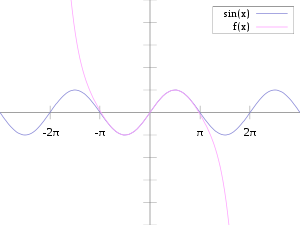
\includegraphics[height = 300pt, width = 225pt]{images/07taylor/taylor-seno-approx-7mo-grado.png}

\esercizio{Calcolate il polinomio di Taylor di grado 5 della funzione esponenziale "scostumata" $10^x$ }
 
% \label{statistica}
\chapter{Statistica}

Mi piacerebbe avvicinare in questo capitolo i neofiti ai vari problemi della statistica, in un modo magari divertente e costruttivo. Credo ci sia ben poco di noioso nella statistica, e anzi che vi siano molti problemi della vita comune che dei buoni fondamenti teorici (meglio pratici) possono aiutare ad affrointare.

Cominciamo con un problema che affligge molti miei amici giocatori di ruolo.  A Dungeons \& Dragons � comune tirare le abilit� con 3 dadi a 6 facce, sommandoli (ottenendo un risultato da 3 a 18). Ora, � pi� facile tirare un 10 o un 18? I problemi coi dadi mi sembrano significativi e anche abbastanza divertenti.
% \label{integrali}
\chapter{Integrali}

TODO(ricc) 
% \label{utilita}
\chapter{Utilit\'a varie}

\citazioneinizioparagrafo{
	Torture numbers, and they'll confess to anything
	}{Gregg Easterbrook}

In questo capitolo sono descritte alcune cose interessanti di pubblica utilit\'a che a mio parere non meritano posto in un capitolo particolare,
ma che devono essere menzionate perch\'e usate da qualche parte.

%%%%%%%%%%%%%%%%%%%%%%%%%%%%%%%%%%%%%%%%%%%%%%%%%%%%%%%
%%% BINOMI NEWTON
\label{binominewton}
\section{Binomi di Newton}
%%%%%%%%%%%%%%%%%%%%%%%%%%%%%%%%%%%%%%%%%%%%%%%%%%%%%%%

I binomi di Newton sono assolutamente fondamentali in statistica e tornano utili quando si affrontano certi problemi con i polinomi. Proviamo a sviluppare a mano $(x+1)^6$:
\begin{equation}
(x+1)^6=x^6+6x^5+15x^4+20x^3+15x^2+6x+1
\end{equation}
Vi potreste chidere: da dove cacchio vengon fuori i numeri $1,6,15,20,15,6,1$?!? Questi numeri vengon fuori dal triangolo di Tartaglia che sicuramente avrete visto allle medie.
Ma esiste un modo matematico rigoroso per definirli, ammesso che sappiate cos'\'e un fattoriale (\refpagref{fattoriale}). Definiamo binomio di Newton $\binom{n}{k}$ (e lo leggiamo "$n$ su $k$") il seguente:
\begin{equation}
\binom{n}{k} \doteq \frac{n!}{n!(n-k)!}
\end{equation}
Il binomio di Newton gode di quattro propriet\'a fondamentali, che chiameremo: {\em unariet\'a} ($\forall n \binom{n}{0}=1$); {\em ennariet\'a} ($\binom{n}{1}=n$),
 {\em simmetria} ($\binom{n}{k}=\binom{n}{n-k}$) e {\em tartagliet\'a} ($\binom{n}{k}+\binom{n}{k+1}=\binom{n+1}{k+1}$). Quest'ultimo \'e la base su cui si basa il triangolo di Tartaglia.
\notaric{guarda che sia corretto!!!}
Io adoro anche il principio di {\em cin-cin} ($\binom{n}{2}=\frac{n(n-1)}{2}$), che \'e il numero di cin-cin che fanno $n$ persone non maleducate che brindano.
Il principio di simmetria vi torner\'a spesso utile quindi CAPITELO! Esempio: $\binom{10}{9}=\binom{10}{1}=10$. Comodo, no?

\begin{equation}
(a+b)^n=
	\binom{n}{0}a^n+\binom{n}{1}a^{n-1}b^1+\binom{n}{2}a^{n-2}b^2+\cdots+\binom{n}{n-1}a^1b^{n-1}+\binom{n}{n}b^n,
\end{equation}
dove:


%%%%%%%%%%%%%%%%%%%%%%%%%%%%%%%%%%%%%%%%%%%%%%%%%%%%%%%
%%% ESPONENTI
\label{esponenti} \section{Gli esponenti}
%%%%%%%%%%%%%%%%%%%%%%%%%%%%%%%%%%%%%%%%%%%%%%%%%%%%%%%

Vorrei perdere qualche riga sull'argomento esponenti poich\'e la gente ha spesso difficolt\'a con essi.
L'esponenziazione \'e un'operazione che si scrive $a^b$ e si legge $a alla b$. In generale (se $b$ \'e intero),
il suo significato \'e: prendi $a$ e moltiplicalo per se stesso tante volte quante \'e $b$: $a^b \doteq \underbrace{a\cdot a \cdot a \ldots \cdot a}_{b volte}$.

Essa gode di alcune interessanti propriet\'a (poniamo $a > 0$):

\begin{eqnarray}
a^{b+c} = a^b \cdot a^c
a^b \cdot c = (a^b)^c
a^0 = 1
a^{-n}=\frac{1}{a^n}
\end{eqnarray}

Alcuni esempi: $2^6=2^32^3=2^42^2$; $10^6=(10^2)^3=(10^3)^2$ (ovvero un milione \'e sia il cubo di cento che il quadrato di mille). 

Si pu\'o esponenziare un valore nullo? $0$ pu\'o essere elevato a qualunque cifra tranne che a $0$ (e far\'a sempre 0), poich\'e $0^0$
introdurrebbe un disturbo nella Forza, pensateci: $(qualunque cosa)^0 = 1$ e $0^{qualunque cosa} = 0$; se facessimo $0^0$ il mondo
esploderebbe trasformandosi in qualcosa di ancora pi\'u incomprensibile\footnote{Almeno secondo la teoria di qualcuno...}. In realt\'a
si pu\'o aggirare il problema per vedere chi vince mettendoci due cose che tendono a zero e facendo il limite. Esempio:
$\lim_{x \rightarrow 0} x^x$, $\lim_{x \rightarrow 0} \sinh(x)^{\sin(x)}$, e cos\'i via.

Si pu\'o esponenziare con una base negativa? Ni. Se l'esponente \'e intero ($0,10,-5,\ldots$) si pu\'o fare, e il risultato
coincide con il valore positivo a meno del segno; il segno sar\'a negativo se il numero \'e dispari, positivo se pari. Tutte 
queste cose le potete vedere da voi sfruttando la definizione.

Veniamo ora alla cosa pi\'u seria: si pu\'o esponenziare con esponente reale? Anzitutto dobbiamo esigere che la base sia non negativa;
togliamo pure la base nulla poich\'e ha poco senso. A questo punto, si pu\'o definire l'esponenziale di base positiva e esponente $razionale$:
\begin{eqnarray}
a^{\frac{p}{q}} \doteq \sqrt[q]{a^p}
\end{eqnarray}

\esempio{
$4^{1.5}=8$; 
$2^{4.5}=16 \sqrt{2}$; 
$10^{0.2}= \sqrt[5]{10}$; 
$9^{0.5}=3$; 
$43^{0.763}=\sqrt[1000]{43^{763}}$; }

Lo so, lo so, vi avevo promesso i reali. Ci arriviamo. A dir il vero, non ho la pi\'u pallida idea di come calcolare una cosa come $2^\pi$. So solo dirvi che esiste e che fa poco pi\'u di $8$, e si avvicina ancor di pi\'u a $2^{3.14}$. Altro dirvi non vo'.



%%%%%%%%%%%%%%%%%%%%%%%%%%%%%%%%%%%%%%%%%%%%%%%%%%%%%%%
%%% FATTORIALE
\label{fattoriale} \section{Il fattoriale}
%%%%%%%%%%%%%%%%%%%%%%%%%%%%%%%%%%%%%%%%%%%%%%%%%%%%%%%

Il fattoriale \'e uno dei pi\'u semplici operatori che si definiscono {\em ricorsivamente}. La definizione \'e questa:
\begin{eqnarray}
fatt(0) \doteq 1\\
fatt(n+1) \doteq n \cdot fatt(n)
\end{eqnarray}
\esempio{I primi valori della serie sono: $1,1,2,6,24,120,720,5040,\ldots$. $fatt(3)=6; fatt(4)=24; fatt(7)=5040$,...}


%%%%%%%%%%%%%%%%%%%%%%%%%%%%%%%%%%%%%%%%%%%%%%%%%%%%%%%
%%% FIBONACCI
\label{fibonacci} \section{I numeri di Fibonacci}
%%%%%%%%%%%%%%%%%%%%%%%%%%%%%%%%%%%%%%%%%%%%%%%%%%%%%%%

I numeri di Fibonacci sono una serie di numeri che potete osservare (almeno per i primi numeri della serie, dato che \'e infinita) su un lato del tetto della chiesa di Notre Dame a Parigi. Ebbene s\'i.

Questa serie \'e definita in modo ricorsivo, esattamente come il fattoriale:

\begin{eqnarray}
fib(0)   \doteq 0\\
fib(1)   \doteq 1\\
fib(n+2) \doteq fib(n)+fib(n+1)
\end{eqnarray}

E' abbastanza semplice da dimostrare che all'infinito hanno un andamento del tipo
$fib(n) \approx \alpha^n$, con $\alpha=\frac{-1+\sqrt{5}}{2} \approx 1.618$
(detto anche numero aureo, noto gi\'a agli antichi greci).


%%%%%%%%%%%%%%%%%%%%%%%%%%%%%%%%%%%%%%%%%%%%%%%%%%%%%%%
%%% GRAFICI CARTESIANI
\label{graficicartesiani} \section{I grafici cartesiani}
%%%%%%%%%%%%%%%%%%%%%%%%%%%%%%%%%%%%%%%%%%%%%%%%%%%%%%%

Nel capitolo funzioni (cap. \refpagref{funzioni}) ho dato per scontata la parte grafica delle funzioni stesse. Credo sia di {\em massima} importanza sapere disegnare un funzione, poich\'e d\'a una comprensione molto pi\'u profonda del problema che ci si sta ponendo. Inoltre, poich\'e i numeri non mentono, consente di accorgersi visivamente di certi errori di calcolo. E' per questo che \'e importante imparare a disgenare funzioni e ad acquisire quel colpo d'occhio che getta un 'ponte' tra equazioni e relativi disegni.

Come si disegna un grafico? Anzitutto prendete due semirette perpendicolari, una che va a nord/su (che chiameremo asse delle $y$)
e una che va a est/destra (asse delle $x$). Poi vi consiglio di fare 4-5 stanghette in ciascuno dei 4 punti cardinali equidistanti
da loro. Se la carta che avete \'e quadrettata, tanto meglio: rendete ogni stanghetta lunga un quadretto. Ogni punto del piano
(inteso come coppia di numeri che indicheremo con $P \equiv (x;y)$) pu\'o essere ora disegnato. Non \'e proprio come disegnare
donne nude, ma vi assicuro che d\'a la sua parte di gusto. Poniamo ad esempio $A \equiv (3,4)$: si legge come "punto $A$ di
coordinate $(3,4)$. Come si disegna? Ebbene, si prende la $x$ (che vale 3) e si va lungo l'asse $x$ (ovvero verso est) di 3 tacche.
Poi si sale a nord di 4 tacche. Attenti ai segni! Il punto $(3;-4)$ indica di andare a est di 3 e a nord di $-4$, quindi di
retrocedere di $4$ tacche a nord, quindi fondamentalmente di andare a sud di $4$, siete d'accordo? Esiste un punto 'raccomandato'
detto origine (che si chiama con la sua iniziale, $O$). Esso \'e sull'intersezione degli assi (cio\'e \'e l'unico punto che non
\'e n\'e a nord n\'e a sud, n\'e a est n\'e a ovest).

\esercizio{Provate a disegnare i $4$ punti $(\pm 3;\pm 4)$ e i due punti $A \equiv (5;0)$ e $B \equiv (0;5)$. Quali sono le distanze di questi punti dall'origine?}

Il bello dei diagrammi cartesiani \'e che per molte cose esiste sia la rappresentazione grafica sia la rappresentazione sotto forma di equazione. Vedere i nessi tra le due cose \'e affascinante per molti, e se siete arrivati a leggere fin qui vuol certamente dire che per voi - se non altro - non \'e soporifero. Prendiamo il concetto di $distanza$: la distanza tra due punti $A\equiv(x_A;y_A);B\equiv(x_B;y_b)$ \'e $graficamente$ la lunghezza del segmento che unisce i due punti, mentre \'e $analiticamente$ il numero: 
\label{distanza euclidea}
\begin{equation}
d_{Eucl} \doteq \sqrt{(x_A-x_B)^2+(y_A-y_B)^2}
\end{equation}
Questa distanza \'e detta euclidea poich\'e i matematici - che non sono mai contenti - ne hanno inventate infinite altre. Io ne conosco altre due, e giusto per divertimento ve ne dico una che chiameremo 'distanza in isolati':
\begin{equation}
d_{Isol} \doteq |x_A-x_B|+|y_A-y_B|
\end{equation}
Il nome derivata dal fatto che questa distanza \'e effettivamente la distanza in chilometri tra due punti supponendo che ci siano grattacieli tra le varie strade, che le strade siano tutte parallele o perpendicolari tra loro,  e che quindi si possa camminare $solo$ in orizzontale o in verticale.

Se disegnate nel diagramma il punto $C\equiv(3;-4)$ e l'origine $O$, potete divertirvi a calcolare la distanza euclidea e 'in isolati' del punto dall'origine. Vengono due bei numerelli, e se non ci credete potete verificarli col righello.

Ora veniamo a qualcosa di pi\'u complicato. Se vi ho insegnato bene a disegnare un punto, credete di potervela cavare a disegnarne 2? E 3? E infiniti?
Credete di no? Beh, pensate che lo fate (quasi) tutti i giorni, ad esempio quando disegnate un cerchio o una lettera dell'alfabeto o un ditone.

Supponiamo che vi dia una funzione (le studierete meglio al cap. \refpagref{funzioni}), ad esempio $y=x^2-2x$. Provate a disegnarla. Sembra difficile?
Non lo \'e, fidatevi. Poich\'e la funzione mangia $x$ e sputa $y$, vi conviene prendere delle $x$ a casaccio (le mie preferite sono le seguenti 5:
$-2;-1;0;1;2$) e vedere quanto vale $f$ in quei 5 punti. Vediamo di fare una tabella:

\begin{tabular}{|r||c|c|c|c|c|c|}
\hline
x & -2 & -1 &  0 & 1  &  2  & \ldots \\
\hline
y &  8 & 3  &  0 & -1  & 0  & \ldots \\
\hline
\end{tabular}

Siete persuasi? Bene, adesso disegnate i 5 punti trovati. Ricordate che avete a disposizione tutti i punti che volete.
Ad esempio, volete disegnarla meglio a destra? Calcolate $f(3)$ e avete un punto in pi\'u a destra. Volete andare a sinistra?
Tentate con $f(-3),f(-4),\ldots$. Avete tutto il tempo che volete. Volete raffinare i punti? Vi consiglio di provare con
$-\frac{1}{2},\frac{1}{2},\frac{3}{2},\ldots$. Volete raffinare ancora di pi\'u? Provate con $0.1,0.2,0.3,\ldots$ ma qui
io non vi aiuto pi\'u perch\'e alla mia et\'a tale precisione \'e superiore a quella delle mie mani ormai...

%%%%%%%%%%%%%%%%%%%%%%%%%%%%%%%%%%%%%%%%%%%%%%%%%%%%%%%
%%% FIBONACCI
\label{ricorsione} \section{La ricorsione}
%%%%%%%%%%%%%%%%%%%%%%%%%%%%%%%%%%%%%%%%%%%%%%%%%%%%%%%

La ricorsione \'e un concetto che ben si sposa con certi aspetti della matematica. Ad esempio,
\'e utile a ocmprendere i fattoriali o i numeri di Fibonacci. In genere una definizione ricorsiva
\'e una definizione di una successione (cap. \refpagref{successioni}) in due parti: si d\'a intanto
la definizione del primo valore, poi si d\'a la definizione di ogni pezzo in funzione del precedente.
Esattamente come i pezzi di un domino, questi valori prendono forma a cascata. Vediamo un esempio 'idiota':
defininiamo la successione $scemo_i$. Anzitutto, la successione $pippo_i$ (ancor prima di sapere che cosa sia)
\'e un insieme di valori esattamente come una funzione: $pippo_0$ di solito \'e il suo primo valore, poi viene
$pippo_1$, poi $pippo_2$, e dopo 1000 valori avremo $pippo_{999}$...

\begin{eqnarray}
pippo_0=10;\\
pippo_{n+1}=pippo_n+3.
\end{eqnarray}

La successione $pippo$ poteva essere definita cos\'i: $pippo_0=10;pippo_1=13;pippo_2=16;pippo_3=19;\ldots$. Ma vi rendete conto che non posso stare qua fino a sera a dirvi tutti i valori? La definizione ricorsiva mi sembra sia una bella comodit\'a, no? Il punto \'e proprio quello.















% \label{numeriprimi}
\chapter{Numeri Primi}

\citazioneinizioparagrafo
  {Mathematicians have tried in vain to this day to discover some
   order in the sequence of prime numbers, and we have reason to believe
   that it is a mystery into which the human mind will never penetrate.}
  {Leonhard Euler}

\TODO{Aggiungi concetti basi sui primi, la loro densita', applicazioni su critttografia, .. e tutta la loro indecidiblita'}
% \chapter{Sull'autore}

Riccardo Carlesso nasce ad Argenta (FE) il 29.12.76.

Sito: %\href{http://www.palladius.it/}{sito pal}.
\end{document}